\documentclass{BitirmeClass}

\usepackage[utf8]{inputenc}
\usepackage[T1]{fontenc}

\usepackage{latexsym,amssymb,amsmath,amsthm,graphicx}
\usepackage{etex}
\usepackage{enumerate}
\usepackage{cite}
\usepackage{tikz}
\usepackage{tabularx}
\usepackage{multirow}
%\usepackage{ctable}
\usepackage{float}
\usepackage{multirow}
\usepackage{caption}
%\usepackage{enumitem}
%\usepackage{uarial}
%\renewcommand{\familydefault}{\sfdefault}
\usepackage[top=3cm, bottom=3cm, left=3cm, right=3cm]{geometry}%%sayfa kenar boşlukları ayarlandı.
\usepackage{times}

\theoremstyle{definition}
\newtheorem{tanim}{Tanım}[section]
\newtheorem{onerme}{Önerme}[section]
\newtheorem{ornek}{Örnek}[section]
\newtheorem{teorem}{Teorem}[section]
\newtheorem{note}{Not}[section]
\newtheorem{sonuc}{Sonuç}[section]
\newtheorem{lemma}{Lemma}[section]
\newtheorem{soru}{Soru}[section]
\newenvironment{ispat}{{\vspace{-10pt} \bf İspat:} }{\hfill $\Box$ \mbox{}}
\newenvironment{cozum}{{\vspace{-10pt} \bf Çözüm:} }{\hfill \mbox{}}

\ToCLineisDotted %% İçindekiler kısmında sayfa numaralarına kadar olan kısım noktalı olsun

\setlength{\fboxsep}{0pt}

\newcommand{\plotPGFfile}{true} % PGF olarak DATA dosyaları çizilsin mi çizilmesin mi? Çizilmez ise dosyadan sadece data okunan kısım atlanıyor, resmin çerçevesi oluşturuluyor...

\author{Melih}{TAŞKIN}
\date{2022}
\teziyoneten{Prof. Dr. Hüsamettin COŞKUN}
%\onaydate{01/01/2014}%  Belli olunca girilecek.
\title{TÜREV}

\BolumBaskani{Prof. Dr. Mustafa KAZAZ}

\ozet{\input ozet.tex}
\ozgecmis{\input ozgecmis.tex}
\tesekkur{\input tesekkur.tex}

\renewcommand{\textfraction}{0.10}
\renewcommand{\topfraction}{0.95}
\renewcommand{\bottomfraction}{0.95}
\renewcommand{\floatpagefraction}{0.35}
\setcounter{totalnumber}{5}

\begin{document}
%giriş bölümü
\chapter{\protect GİRİŞ}
Türev bir fonksiyonun değişme hızını ölçer ve analizdeki en önemli fikirlerden biridir. Türevler hız ve ivme hesaplamada, bir hastalığın yayılma
oranını tahmin etmede, verimliliği maksimize edecek şekilde üretim seviyesini belirlemede, silindirik bir kutunun ideal boyutlarını bulmada, tarih öncesi bir sanat eserinin
yaşını belirlemede ve bir çok başka uygulamalar için kullanılır. Bu bölümde, türevleri
hesaplamayı kolaylaştıracak yöntemler geliştireceğiz ve türevlerin karmaşık fonksiyonlara
yaklaşımda nasıl kullanılacağını öğreneceğiz

%ana bölüm
\chapter{\protect FONKSİYON OLARAK TÜREV}
\section{\protect Türev Fonksiyonu} \label{bolumetiketi}
\begin{tanim}
	Bir $f(x)$ fonksiyonunun $x$ değişkenine göre türevi, $x$'teki değeri
\begin{equation*}
	f'(x) = \lim_{h \rightarrow 0} \frac{f(x + h)-f(x)}{h}
\end{equation*}
	olan(limitin bulunması koşuluyla) $f'$ fonksiyonudur.
\end{tanim}
	Bağımsız değişken $x$'e göre türev aldığımızı belirtmek için, tanımdan basitçe $f$ yerine $f(x)$ notasyonunu kullanırız. $f'$'nin tanım kümesi, $f'$'nin tanım kümesinde limitin var olduğu noktaların kümesi, $f'$'nin tanım kümesiyle aynı veya daha küçük olabilir. Belirli bir $x$ için varsa, $f'$'nin $x$'te bir türevi vardır(türevlenebilir) deriz. $f'$'nin tanım kümesinin her noktası için $f'$ varsa $f$'ye türevlenebilir deriz.\\
	Eğer $z=x+h$ yazarsak $h=z-x$ olur ve ancak ve yalnız $z\rightarrow x$ ise $h\rightarrow 0$dır. Bu nedenle, türevin bir eşdeğer tanımı şekil 2.1den de anlaşılabileceği üzere aşağıdaki gibidir.
\section{\protect Türev İçin Alternatif Bir Formül }\label{bolumetiketi}
\begin{equation*}
	f'(x) = \lim_{z \rightarrow x} \frac{f(z)-f(x)}{z-x}
\end{equation*}
\begin{figure}[H]	
	\centering
	\includegraphics[width=0.3\linewidth]{şekil-1.png}
	\caption{Bir $f$ fonksiyonunun türevi için fark oranını yazma şekli ilgilendğimiz noktaları nasıl işaretlediğimize bağlıdır.}
	\label{fig:ornekresim}
\end{figure}
\section{\protect Tanımı Kullanarak Türev Hesaplama}\label{bolumetiketi}
Bir türevin hesaplama işlemine türev alma denir. Türev almanın $y = f(x)$ fonksiyonuna uygulanan bir işlem olduğunu vurgulamak için $f'(x)$ türevini göstermenin bir başka yolu olan
\begin{equation*}
	 \frac{d}{dx}f(x)
\end{equation*}
notasyonunu kullanırız. Örneğin,
\begin{equation*}
	 \frac{d}{dx}\left(\frac{3}{2}x-4\right) = \frac{3}{2}
\end{equation*}
ve
\begin{equation*}
	 \frac{d}{dx}\left(\frac{1}{x}\right) = -\frac{1}{x^2}
\end{equation*}
gibidir. Aşağıdaki örnekler, türevin tanımının nasıl uygulanacağına yöneliktir. Örneklerin çözümleri adım adım olup, okuyucunun kolayca anlaması amaçlanmıştır.
\begin{ornek}
$f(x) = \frac{x}{x-1}$ fonksiyonunun türevini alın.
\end{ornek}
\begin{cozum}
	\begin{equation*}
	\begin{split}
		f(x)  &=\frac{x}{x-1}\\
		f(x+h)  &=\frac{(x+h)}{(x+h)-1}\\
		f'(x) & =\lim_{h \rightarrow 0}\frac{f(x+h)-f(x)}{h}\\
		& = \lim_{h \rightarrow 0}\frac{\frac{x+h}{x+h-1}-\frac{x}{x-1}}{h}\\
		& = \lim_{h \rightarrow 0}\frac{1}{h}.\frac{(x+h)(x-1)-x(x+h-1)}{(x+h-1)(x-1)}\\
		& = \lim_{h \rightarrow 0}\frac{1}{h}.\frac{-h}{(x+h-1)(x-1)}\\
		& = \lim_{h \rightarrow 0}\frac{-1}{(x+h-1)(x-1)}=\frac{-1}{(x-1)^2}\\
	\end{split}
\end{equation*}
\end{cozum}
\begin{ornek}
(a) $x>0$ için $y=\sqrt{2}$'in türevini bulunuz.\\
(b) $y=\sqrt{x}$ eğrisinin $x=4$'teki teğetini bulunuz.
\end{ornek}
\begin{cozum}
(a) $f'$'yü hesaplamak için eşdeğer formu kullanırız:
\begin{equation*}
\begin{split}
		f'(x)  & =\lim_{z \rightarrow x}\frac{f(z)-f(x)}{z-x}\\
		        & =\lim_{z \rightarrow x}\frac{\sqrt{z}-\sqrt{x}}{z-x}\\
		        & =\lim_{z \rightarrow x}\frac{\sqrt{z}-\sqrt{x}}{(\sqrt{z}-\sqrt{x})(\sqrt{z}+\sqrt{x})}\\
		        & =\lim_{z \rightarrow x}\frac{1}{\sqrt{z}+\sqrt{x}}=\frac{1}{2\sqrt{x}}\\
\end{split}
\end{equation*}
(b) $x=4$'te eğrinin eğimi
\begin{equation*}
	f'(4)=\frac{1}{2\sqrt{4}}=\frac{1}{4}
\end{equation*}
tür. Teğet, $(4,2)$ noktasından $1/4$ eğimiyle geçen doğrudur.\\
\begin{equation*}
\begin{split}
	 y &= 2 + \frac{1}{4}(x-4)\\
	 y &= \frac{1}{4}x + 1\\
\end{split}
\end{equation*}
\end{cozum}
\section{\protect Gösterim}\label{bolumetiketi}
Bağımsız değişkenin $x$ ve bağlı değişken $y$ olduğu bir $y=f(x)$ fonksiyonunun türevini göstermenin bir çok yolu vardır. Bazı yaygın alternatif gösterimler şunlardır:
\begin{equation*}
f'(x)= y' = \frac{dy}{dx}=\frac{df}{dx} = \frac{d}{dx}f(x) = D(f)(x) =D_x f(x)
\end{equation*}
$d/dx$ ve $D$ sembolleri türev almanın bir işlem olduğunu belirtirler ve türev alma operatörleri olarak adlandırılırlar. $dy/dx$'i "$y$'nin ve $x$'e göre türevi" olarak, $df/dx$ ve $(d/dx)f(x)$'i de "$f$'nin $x$'e göre türevi olarak okuruz. "Üs" gösterimleri $y'$ ve $f'$ Newton'un türev için kullandığı gösterimlerden gelir. $d/dx$ gösterimleri Leibniz'in kullandıklarıyla aynıdır. $\displaystyle \frac{dy}{dx}$ sembolü bir oran olarak görülmemelidir. \\
$D(f)$ notasyonunu, türev fonksiyonu $f'$ yerine $f$ fonksiyonunun tanım kümesi ile karıştırmama konusunda dikkatli olun. Farklılık içerikten anlaşılmalıdır.\\
Bir türevin belirli bir $x=a$ sayısındaki değerini belirtmek için şu notasyonları kullanırız:
\begin{equation*}
f'(a) = \frac{dy}{dx} |_{x=a} = \frac{df}{dx} |_{x=a} = \frac{d}{dx}f(x) |_{x=a}
\end{equation*}
Örneğin, örnek 2.0.2de şunları yazabilirdik;
\begin{equation*}
f'(4) = \frac{dy}{dx}\sqrt{x} |_{x=4} = \frac{1}{2\sqrt{x}} |_{x=4} = \frac{1}{2\sqrt{4}}=\frac{1}{4}
\end{equation*}
Bazen bir ifadeyi hesaplamak için dik çizgi "$|$" yerine köşeli parantez "$]$" kullanırız. \\
\section{\protect Türevin Grafiğini Çizmek}\label{bolumetiketi}
Eğimleri $f$'nin grafiğinden tahmin ederek, çoğunlukla $y=f(x)$'in türevinin makul bir çizimini yapabiliriz. Yani, $xy$-düzleminde $(x,f'(x))$ noktalarını işaretler ve düzgün bir eğri ile onları birleştiririz. Bu eğri $y=f'(x)$'i temsil eder.
\begin{ornek}
Şekil 2.2a'daki $y=f(x)$ fonksiyonunun türevini çizin.
\end{ornek}
\begin{cozum} Sık aralıklarla $f$ grafiğine teğetler çizer ve teğetlerin eğimlerinden $f'(x)$'in bu noktalardaki değerlerini buluruz. Bunlara karşılık gelen $(x,f'(x))$ çiftlerini işaretler ve bunları Şekil 2.2b'de yapıldığı gibi düzgün bir eğriyle birleştiririz.
	

$y=f'(x)$ grafiğinden neler öğrenebiliriz? İlk bakışta şunlar görülebilir:\\
1.$f$'nin değişim oranının pozitif, negatif veya sıfır olduğu yerler;\\
2.Herhangir bir $x$ değerindeki büyüme oranının kabaca büyüklüğü ve bu büyüklüğün $f(x)$'in büyüklüğüyle ilişkisi;\\
3.Değişim oranının kendisinin artıp artmadığı.
\begin{figure}[H]
	\centering
	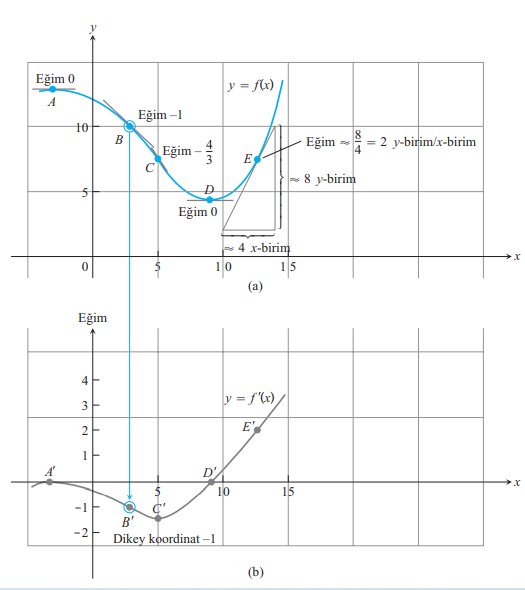
\includegraphics[width=0.7\linewidth]{turevcizim.png}
	\caption{(a)'daki $y=f(x)$ grafiğinin eğimlerini işaretleyerek (b)'deki $y=f'(x)$'in grafiğini çizdik. Mesela, $B'$'nin dikey koordinatı $B$'deki eğimidir. $f'$'in grafiği $f$'nin eğiminin $x$ ile nasıl değiştiğinin görsel kaydıdır.}
	\label{fig:ornekresim}
\end{figure}
\end{cozum}
\section{\protect Bir Aralıkta Türevlenebilirlik; Tek Taraflı Türevler}\label{bolumetiketi}
Bir $y=f(x)$ fonksiyonunun (sonlu veya sonsuz) bir açık aralığın her noktasında türevi varsa, $f(x)$'e bu aralıkta türevlenebilir denir. Bir $[a,b]$ kapalı aralığının içi $(a,b)$ açık aralığında türevlenebilirse ve uç noktalarında
\begin{equation*}
	\lim_{h \rightarrow 0^+}\frac{f(a+h)-f(a)}{h} 
\end{equation*}\\
\begin{equation*}
	\lim_{h \rightarrow 0^-}\frac{f(b+h)-f(b)}{h}
\end{equation*}
limitleri varsa, [a,b] kapalı aralığında türevlenebilirdir. \\
	Bir fonksiyonun tanım aralığının herhangi bir noktasında sağdan ve soldan türevler tanımlanabilir. Tek taraflı ve iki taraflı limitler arasındaki ilişki bu türevler için de geçerlidir. Bir fonksiyonun, ancak ve yalnız bir noktada sağdan ve soldan türevleri varsa ve bu tek taraflı türevler eşitse o noktada türevi olabilir.
\begin{ornek}
$y=|x|$ Fonksiyonu Orijinde Türevlenebilir Değildir

$y=|x|$ fonksiyonunun $(-\infty,0)$ ve $(0,\infty)$ aralıklarında türevlenebilir olduğunu, fakat $x=0$'da türevinin bulunmadığını gösterin.
\end{ornek}
\begin{cozum} Orijinin sağında,
	\begin{equation*}
		\frac{d}{dx}(|x|) =\frac{d}{dx}(x)=1,
		\left(\frac{d}{dx}(mx+b)=m, |x| = x\right)
	\end{equation*}
ve solunda
	\begin{equation*}
		\frac{d}{dx}(|x|) =\frac{d}{dx}(-x)=-1,
		\left(\frac{d}{dx}(mx+b)=m, |x| = -x\right)
	\end{equation*}
bulunur(Şekil 2.3). Orijinde türev olamaz, çünkü tek taraflı türevler bu noktada farklıdır:
	$0$'da $|x|$'in sağdan türevi
		\begin{equation*}
		\begin{split}
		   & =\lim_{h \rightarrow 0^+}\frac{|0+h|-|0|}{h}=\lim_{h \rightarrow 0^+}\frac{|h|}{h}\\
		   &=  \lim_{h \rightarrow 0^+}\frac{h}{h}\\
		   &=  \lim_{h \rightarrow 0^+}1=1
		\end{split}
		\end{equation*}
	$0$'da $|x|$'in soldan türevi	
		\begin{equation*}
		\begin{split}
		   & =\lim_{h \rightarrow 0^-}\frac{|0+h|-|0|}{h}=\lim_{h \rightarrow 0^-}\frac{|h|}{h}\\
		   &=  \lim_{h \rightarrow 0^-}\frac{-h}{h}\\
		   &=  \lim_{h \rightarrow 0^-}-1=-1
		\end{split}
		\end{equation*}	
\begin{figure}[H]
	\centering
	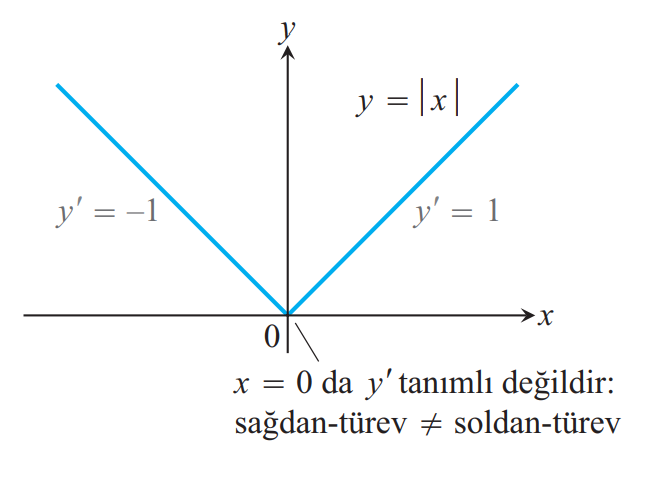
\includegraphics[width=0.5\linewidth]{mutlakxturev.png}
	\caption{$y=|x|$ fonksiyonu, grafiğinde bir "köşenin" bulunduğu orijinde türevlenemez.}
	\label{fig:ornekresim}
\end{figure}
\end{cozum}
\section{\protect Ne Zaman Bir Fonksiyonun Bir Noktada Türevi Yoktur?}\label{bolumetiketi}
Bir fonksiyonun grafiğindeki $P(x_0,f(x_0))$'dan ve yakınındaki bir $Q$ noktasından geçen kirişlerin eğimleri, $Q$ $P$'ye yaklaşırken bir limite gidiyorsa, fonksiyonun $x_0$ noktasında türevi vardır. $Q$  $P$'ye giderken, kirişler bir limit konuma ulaşamadıklarında veya dikey olduklarında, türev bulunmaz. Böylece, türevlenebilirlik bir $f$ fonksiyonunun grafiği üzerinde "düzgünlük" koşuludur. Grafiği düzgün olan bir fonksiyonun ise birkaç sebepten dolayı bir noktada türevi bulunmayabilir, grafiğinde aşağıdaki durumlar bulunuyorsa türevi yoktur:
\begin{figure}[H]
	\centering
	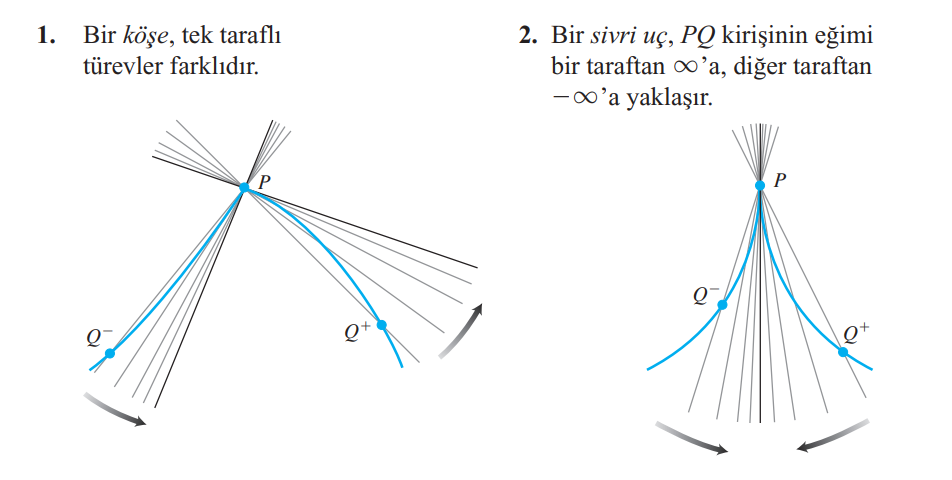
\includegraphics[width=0.75\linewidth]{turevyok1.png}
	\label{fig:ornekresim}
\end{figure}
\begin{figure}[H]
	\centering
	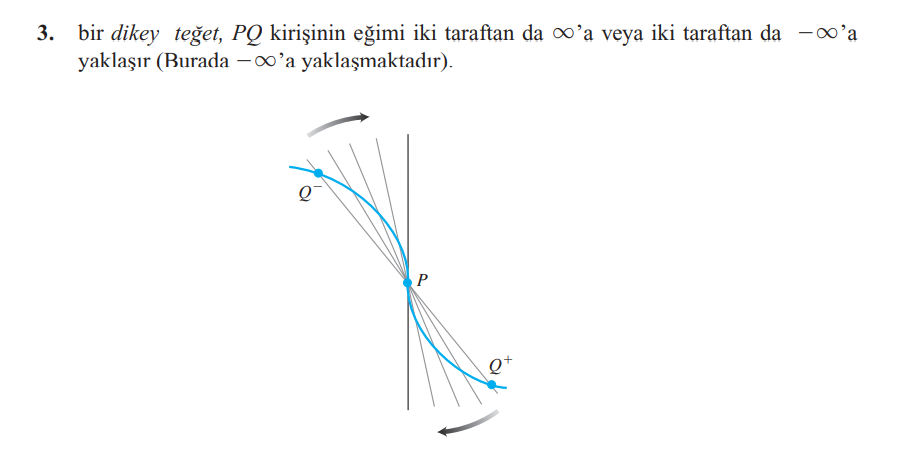
\includegraphics[width=0.75\linewidth]{turevyok2.png}
	\label{fig:ornekresim}
\end{figure}
\begin{figure}[H]
	\centering
	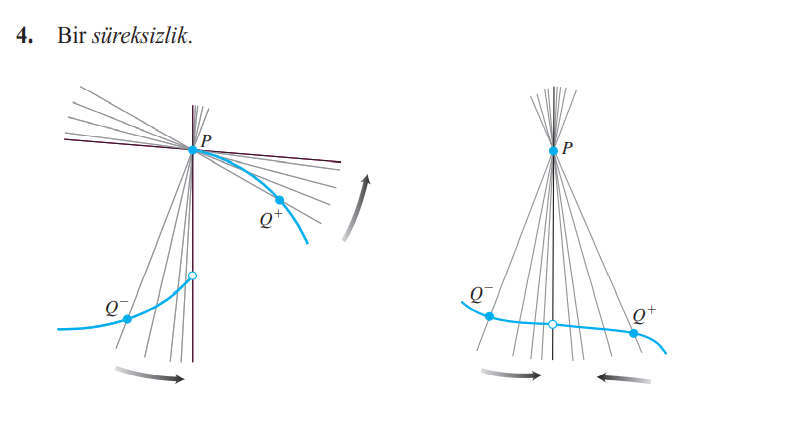
\includegraphics[width=0.75\linewidth]{turevyok3.png}
	\label{fig:ornekresim}
\end{figure}
\section{\protect Türevlenebilir Fonksiyonlar Süreklidir}\label{bolumetiketi}
Bir fonksiyon, türevinin bulunduğu her noktada süreklidir
\begin{teorem}
	$f$'nin $x=c$'de bir türevi varsa, $f$ fonksiyonu $x=c$'de süreklidir.
\end{teorem}
İspat: $f'(c)$'nin var olduğu verilmiştir, $\lim_{x \rightarrow c}f(x) = f(c)$ veya buna eşdeğer olarak $\lim_{h \rightarrow 0}f(c+h)=f(c)$ olduğunu göstermemiz gerekir. $h\ne0$ ise,
		\begin{equation*}
		\begin{split}
		  f(c+h) & = f(c) + (f(c+h)-f(c))\\
		   &=  f(c)+\frac{f(c+h)-f(c)}{h}.h
		\end{split}
		\end{equation*}	
yazılabilir.\\
	
Şimdi, $h \rightarrow 0$ iken limit alalım.
		\begin{equation*}
		\begin{split}
		 \lim_{h \rightarrow 0}f(c+h) &= \lim_{h \rightarrow 0}f(c) +\lim_{h \rightarrow 0}\frac{f(c+h)-f(c)}{h}\lim_{h \rightarrow 0}h\\
		&=f(c)+f'(c).0\\
		&=f(c)+0\\
		&=f(c).
		\end{split}
		\end{equation*}	
bulunur.\\
	Tek taraflı limitlerdeki ifadelerin benzerleri $f$'nin $x=c$'de bir taraftan (sağdan veya soldan) türevi varsa, $f$'nin $x=c$'de o taraftan sürekli olduğunu gösterir. Bu teorem şunu söyler: bir fonksiyonun bir noktada süreksizliği varsa fonksiyon o noktada türevlenebilir olamaz. Bu teoremin tersi  doğru olmak zorunda değildir. Örnek 2.6.1'de verdiğimiz $|x|$ fonksiyonu orijinde süreklidir fakat türevlenebilir değildir.\\
\section{\protect Türevlerin Ara Değer Özelliği}\label{bolumetiketi}
İlk olarak, Fransız matematikçi Jean Gaston Darboux(1842-1917) tarafından, 1875 yılında ispat edilen aşağıdaki teoremden görülebileceği gibi, her fonksiyon bir başka fonksiyonun türevi olamaz.
\begin{teorem}
	$a$ ve $b$, $f$'nin türevli olduğu bir aralıkta iki noktaysa, $f',f'(a)$ ile $f'(b)$ arasındaki her değeri alır.
\end{teorem}

\chapter{\protect TÜREV KURALLARI}
Bu bölüm, fonksiyon çeşitlerinden çok büyük bir bölümünün türevlerini almamızı sağlayan birkaç kural tanıtmaktadır. Bu kıralları burada ispat etmekle, her seferinde tanımı uygulamadan fonksiyonların türevlerini alabileceğiz
\section{\protect Kuvvetler, Katlar, Toplamlar ve Farklar} \label{bolumetiketi}
Türev almanın birinci kuralı sabit her fonksiyonun türevi sıfır olduğudur.
\subsection{\protect Bir Sabit Fonksiyonun Türevi}
$f$ sabit fonksiyon $f(x)=c$ ise,
	\begin{equation*}
		\frac{df}{dx}=\frac{d}{dx}(c)=0
\end{equation*}
olur.\\
İspat: Türev tanımını, sonuçları sabit c değeri olan $f(x)=c$ fonksiyonuna uygularız. Her $x$ değerinde
	\begin{equation*}
		f'(x)= \lim_{h \rightarrow 0} \frac{f(x+h)-f(x)}{h}=\lim_{h \rightarrow 0} \frac{c-c}{h}=\lim_{h \rightarrow 0} \frac{0}{h} = \lim_{h \rightarrow 0}0=0
	\end{equation*}
olduğunu buluruz.
\begin{ornek}
$f$'nin değeri sabit ve $f(x)=8$ ise,
	\begin{equation*}
		\frac{df}{dx}=\frac{d}{dx}(8)=0
	\end{equation*}
dır.Benzer şekilde,
	\begin{equation*}
		\frac{d}{dx}\left(-\frac{\pi}{2}\right)=0
	\end{equation*}
	\begin{equation*}
		\frac{d}{dx}\left(\sqrt{3}\right)=0
	\end{equation*}
dır.
\end{ornek}



\subsection{\protect Pozitif Tamsayılar İçin Kuvvet Kuralı}
$n$ pozitif bir tamsayı ise,
	\begin{equation*}
		\frac{d}{dx}x^n=nx^{n-1}
	\end{equation*}	
olur.\\
Pozitif tam sayılar için kuvvet kuralının birinci ispatı
	\begin{equation*}
		z^n-x^n = (z-x)(z^{n-1}+z^{n-2}x+...+zx^{n-2}+x^{n-1})
	\end{equation*}
formülü, sağ taraf çarpılarak sağlanabilir. Böylece, türev tanımının alternatif formundan
	\begin{equation*}
		\begin{split}
		f'(x) &= \lim_{z \rightarrow x}\frac{f(z)-f(x)}{z-x}=\lim_{z \rightarrow x}\frac{z^n-x^n}{z-x}\\
		&= \lim_{z \rightarrow x}(z^{n-1}+z^{n-2}x+...+zx^{n-2}+x^{n-1})\\
		&=nx^{n-1}
	\end{split}
		\end{equation*}
bulunur.\\
Pozitif tam sayılar için kuvvet kuralının ikinci ispatı: $f(x) = x^n$ise, $f(x+h)=(x+h)^n$ olur.$n$ pozitif bir tam sayı olduğundan, Binom Teoremine göre $(x+h)^n$ yi açarak
	\begin{equation*}
		\begin{split}
		f'(x) &= \lim_{h \rightarrow 0}\frac{f(x+h)-f(x)}{h}=\lim_{h \rightarrow 0}\frac{(x+h)^n-x^n}{h}\\
		&= \lim_{h \rightarrow 0}\frac{\left[x^n+nx^{n-1}h+\frac{n(n-1)}{2}x^{n-2}h^2+...+nxh^{n-1}+h^n\right]-x^n}{h}\\
		&= \lim_{h \rightarrow 0}\frac{nx^{n-1}h+\frac{n(n-1)}{2}x^{n-2}h^2+...+nxh^{n-1}+h^n}{h}\\
		&= \lim_{h \rightarrow 0}\left[nx^{n-1}+\frac{n(n-1)}{2}x^{n-2}h+...+nxh^{n-2}+h^{n-1}\right]\\
		&= nx^{n-1}
	\end{split}
		\end{equation*}
buluruz.
\subsection{\protect Sabitle Çarpım Kuralı}
$u$ $x$'in türevlenebilir bir fonksiyonu ve $c$ bir sabit ise,
	\begin{equation*}
		\frac{d}{dx}(cu) = c \frac{du}{dx}
	\end{equation*}
olur.\\
Özel olarak, n pozitif bir tamsayı ise,
	\begin{equation*}
		\frac{d}{dx}(cx^n) = cnx^{n-1}
	\end{equation*}
olur. İspat: 
	\begin{equation*}
	\begin{split}
		\frac{d}{dx}(cu)&=\lim_{h \rightarrow 0}\frac{cu(x+h)-cu(x)}{h} \\
		&=c\lim_{h \rightarrow 0}\frac{u(x+h)-u(x)}{h}\\
		&=c \frac{du}{dx}\\
	\end{split}
	\end{equation*}
\begin{ornek}
	\begin{equation*}
	\frac{d}{dx}(3x^2)=3.2x=6x
	\end{equation*}
türev formülü $y=x^2$ grafiğini her $y$ koordinatını 3 ile çarparak yeniden ölçeklersek, her noktada eğimi 3 ile çarpacağımızı söyler(Şekil 3.1).
\begin{figure}[H]
	\centering
	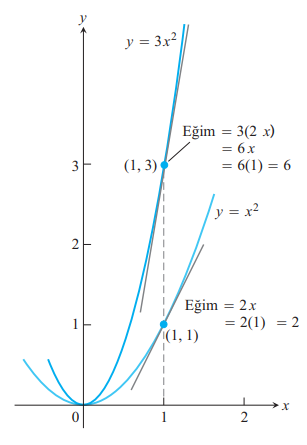
\includegraphics[width=0.5\linewidth]{kural3.png}
	\caption{$y=x^2$ ve $y=3x^2$ grafikleri.$y$- koordinatlarını üçle çarpmak eğimi üç katına çıkarır.}
	\label{fig:ornekresim}
\end{figure}
Yararlı bir özel durum: Türevlenebilir bir fonksiyonun negatifinin türevi fonksiyonun türevinin negatifidir. Sabitle çarpım kuralında c= -1 alırsak
	\begin{equation*}
	\frac{d}{dx}(-u)=\frac{d}{dx}(-1.u)=-1\frac{d}{dx}(u) = -\frac{du}{dx}
	\end{equation*}
elde ederiz.
\end{ornek}
\subsection{\protect Türev Toplama Kuralı}
$u$ ve $v$ $x$'in türevlenebilir fonksiyonları ise, toplamları $u + v$ her ikisinin de türevlenebildiği her noktada türevlenebilirdir. Bu şekildeki noktalarda
	\begin{equation*}
	\frac{d}{dx}(u+v) = \frac{du}{dx}+\frac{dv}{dx}
	\end{equation*}
olur.\\
İspat: Türev tanımını $f(x)= u(x) + v(x)$'e uygularız.
	\begin{equation*}
	\begin{split}
		\frac{d}{dx}[u(x) + v(x)]&=\lim_{h \rightarrow 0}\frac{[u(x+h)+v(x+h)]-[u(x)+v(x)]}{h} \\
		&=\lim_{h \rightarrow 0}\left[\frac{u(x+h)-u(x)}{h}+\frac{v(x+h)-v(x)}{h}\right]\\
		&=\lim_{h \rightarrow 0}\frac{u(x+h)-u(x)}{h}+\lim_{h \rightarrow 0}\frac{v(x+h)-v(x)}{h}=\frac{du}{dx}+\frac{dv}{dx}
	\end{split}
	\end{equation*}
Toplam kuralını sabitle çarpım kuralıyla birleştirirsek, türevlenebilen fonksiyonların farkının türevinin, türevlerinin farkı olduğunu söyleyen fark kuralını elde ederiz
	\begin{equation*}
	\frac{d}{dx}(u-v) = \frac{d}{dx}[u+(-1)v]=\frac{du}{dx}+(-1)\frac{dv}{dx}=\frac{du}{dx}-\frac{dv}{dx}
	\end{equation*}
Toplam kuralı ayrıca, toplamda sonlu sayıda fonksiyon bulunması şartıyla, iki fonksiyondan fazla fonksiyonun toplamı için de geçerlidir. $u_1,u_2,...,u_n$ $x$'te türevlenebiliyorsa, $u_1+u_2+...+u_n$ de türevlenebilirdir ve şu sonucu buluruz:
	\begin{equation*}
	\frac{d}{dx}(u_1+u_2+...+u_n)=\frac{du_1}{dx}+\frac{du_2}{dx}+...+\frac{du_n}{dx}
	\end{equation*}
ve bulunan bu sonuç tümevarım metoduyla ispatlanır.
\begin{ornek}Bir Toplamın Türevi:
	\begin{equation*}
	\begin{split}
		y&=x^4 + 12x \\
		\frac{dy}{dx}&=\frac{d}{dx}(x^4)+\frac{d}{dx}(12x)\\
		&=4x^3+12
	\end{split}
	\end{equation*}
\end{ornek}
\begin{ornek} Bir Polinomun Türevi:
	\begin{equation*}
	\begin{split}
		y&=x^3+\frac{4}{3}x^2-5x+1 \\
		\frac{dy}{dx}&=\frac{d}{dx}\left(x^3\right)+\frac{d}{dx}\left(\frac{4}{3}x^2\right)-\frac{d}{dx}\left(5x\right)+\frac{d}{dx}\left(1\right)\\
		&=3x^2+\frac{8}{3}x-5
	\end{split}
	\end{equation*}
Bu örnekten görebileceğiniz gibi, herhangi bir polinomun türevini terim terim alabileceğimize dikkat edin.
\end{ornek}
\begin{ornek}Yatay Teğetleri Bulma:\\
$y=x^4 - 2x^2+2$ eğrisinin yatay teğeti var mıdır? Varsa, nerededir?
\end{ornek}
\begin{cozum}
	Varsa, yatay teğetler eğiminin sıfır olduğu noktalarda bulunur yani $dy/dx = 0$ olmalıdır. Şu halde,
	\begin{equation*}
		\frac{dy}{dx}=\frac{d}{dx}(x^4-2x^2+2)=4x^3-4x
	\end{equation*}dir.\\
Şimdi, $x$ için $\frac{dy}{dx}=0$ denklemini çözelim.
	\begin{equation*}
	\begin{split}
	4x^3-4x&=0\\
	4x(x^2-1)&=0\\
	x&=0,1,-1
	\end{split}
	\end{equation*}
$y=x^4 - 2x^2+2$ eğrisinin $x=0,1$ve$-1$'de yatay teğetleri vardır. Eğri üzerinde bunlara karşılık gelen noktalar (0,2),(1,1) ve (-1,1) noktalarıdır.
\end{cozum}

\subsection{\protect Çarpım Kuralı}
İki fonksiyonun toplamının türevi türevlerinin toplamına eşitken, iki fonksiyonun çarpımlarının türevi türevlerinin çarpımına eşit değildir. Örneğin,
	\begin{equation*}
		\frac{d}{dx}(x).\frac{d}{dx}(x)=1.1=1
	\end{equation*}iken
	\begin{equation*}
		\frac{d}{dx}(x.x)=\frac{d}{dx}(x^2)=2x
	\end{equation*}
bulunur. İki fonksiyonun çarpmının türevi şimdi açıklayacağımız gibi iki çarpımın toplamına eşittir.
	\begin{equation*}
		\frac{d}{dx}(uv)=u\frac{dv}{dx}+v\frac{du}{dx}
	\end{equation*}
olur.\\
$uv$ çarpımının türevi $u$ kere $v$'nin türevi artı $v$ kere $u$'nun türevidir. Üslü gösterimle, $(uv)'=uv'+vu'$ yazılır. Fonksiyon notasyonu ile
	\begin{equation*}
		\frac{d}{dx}[f(x)g(x)]=f(x)g'(x)+g(x)f'(x).
	\end{equation*}
yazılabilir.\\
İspat: \begin{equation*}
		\frac{d}{dx}(uv)=\lim_{h \rightarrow 0} \frac{u(x+h)v(x+h)-u(x)v(x)}{h}
	\end{equation*}
Bu kesri $u$ ve $v$'nin türevlerinin farklar oranını içeren bir hale dönüştürmek için kesrin pay kısmına $u(x+h)$ ekler çıkarırız.
\begin{equation*}
\begin{split}
			\frac{d}{dx}(uv)&=\lim_{h \rightarrow 0}\frac{u(x+h)v(x+h)-u(x+h)v(x)+u(x+h)v(x)-u(x)v(x)}{h}\\
				&=\lim_{h \rightarrow 0}\left[u(x+h)\frac{v(x+h)-v(x)}{h}+v(x)\frac{u(x+h)-u(x)}{h}\right]\\
				&=\lim_{h \rightarrow 0}u(x+h).\lim_{h \rightarrow 0}\frac{v(x+h)-v(x}{h}+\lim_{h \rightarrow 0}v(x).\lim_{h \rightarrow 0}\frac{u(x+h)-u(x)}{h}
\end{split}
\end{equation*}
$h$ sıfıra yaklaşırken, $u(x+h)u(x)$'e yaklaşır, çünkü $u$, $x$'te türevlenebildiği için, $x$'te süreklidir. İki kesir de $dv/dx$ ve $du/dx$'in $x$'teki değerlerine yaklaşır. Kısacası
\begin{equation*}
 	\frac{d}{dx}(uv)= u \frac{dv}{dx} + v \frac{du}{dx}
\end{equation*}
bulunur.
\begin{ornek}Çarpım Kuralını Kullanma:\\
\begin{equation*}
		y=\frac{1}{x}\left(x^2+\frac{1}{x}\right)
\end{equation*}		
fonksiyonun türevini bulun.
\end{ornek}	
\begin{cozum}
$u=1/x$ ve $v=x^2+(1/x)$ ile çarpım kuralını uygularız.
	\begin{equation*}
	\begin{split}
\frac{d}{dx}\left[\frac{1}{x}\left(x^2+\frac{1}{x}\right)\right]&=\frac{1}{x}\left(2x-\frac{1}{x^2}\right)+\left(x^2+\frac{1}{x}\right)\left(-\frac{1}{x^2}\right)\\
			&=2-\frac{1}{x^3}-1-\frac{1}{x^3}\\
			&=1-\frac{2}{x^3}
	\end{split}
	\end{equation*}
\end{cozum}

\begin{ornek} Sayasal Değerlerden Türev:\\
$y=uv$ $u$ ve $v$ fonksiyonlarının çarpımı olsun.
 	\begin{equation*}
u(2)=3,	u'(2)=-4, v(2)=1, v'(2)=2
	\end{equation*}
ise $y'(2)$'yi bulun.
\end{ornek}

\begin{cozum}
	\begin{equation*}
y' = (uv)' = uv'+vu'
	\end{equation*}
şeklinde yazılmış olan çarpım kuralından 
	\begin{equation*}
	\begin{split}
	y'(2) &=u(2)v'(2)+v(2)u'(2)\\
	&=(3)(2) + (1)(-4)=6-4=2
	\end{split}
	\end{equation*}
buluruz.
\end{cozum}
\begin{ornek} Bir Çarpımın Türevini İki Yolla Bulma:\\
$y=(x^2)(x^3+3)$ fonksiyonunun türevini bulun.
\end{ornek}
\begin{cozum}
	(a) Çarpım kuralından, $u=x^2+$ ve $v=x^3+3$, alırsak
	\begin{equation*}
	\begin{split}
	\frac{d}{dx}[(x^2+1)(x^3+3)]&=(x^2+1)(3x^2)+(x^3+3)(2x)\\
		&=3x^4+3x^2+2x^4+6x\\
		&=5x^4+3x^2+6x.
	\end{split}
	\end{equation*}
	(b)Bu özel çarpımın türevi ayrıca,$y$'nin orijinal ifadesindeki çarpımları yapıp ortaya çıkan polinomun türevini almakla da bulunabilir:
	\begin{equation*}
	\begin{split}
	y&=(x^2+1)(x^3+3)=x^5+x^3+3x^2+3\\
	\frac{dy}{dx}&=5x^4+3x^2+6x
	\end{split}
	\end{equation*}
Bu ilk sonucumuzla uyumludur.
\end{cozum}
İki türevlenebilir fonksiyonun çarpımının türevi türevlerinin çarpımları olmadığı gibi, iki fonksiyonun bölümünün türevi de türevlerinin bölümü değildir. \\



\subsection{\protect Bölüm Kuralı}
$u$ ve $v$ $x$'te türevlenebilir ve $v(x)\ne 0$ ise, $u/v$ bölümü $x$'te türevelenebilir ve sonuç
	\begin{equation*}
	\dfrac{d}{dx}\left( \dfrac{u}{v}\right) =\dfrac{v\dfrac{du}{dx}-u\dfrac{dy}{dx}}{v^{2}}
	\end{equation*}
olur.\\
Fonksiyon notasyonu ile:
	\begin{equation*}
		\dfrac{d}{dx}\left[ \dfrac{f\left( x\right) }{g\left( x\right) }\right] =\dfrac{g\left( x\right) f'\left( x\right) -f\left( x\right) g'\left( x\right) }{g^{2}\left( x\right) }
	\end{equation*}
\begin{ornek} $\displaystyle y=  \frac{t^2-1}{t^2+1}$ fonksiyonunun türevini bulun.
\end{ornek}
\begin{cozum}
	$u=t^2-1$ ve $v=t^2+1$ alarak bölüm kuralını uygularız:
	\begin{equation*}
	\begin{split}
	\frac{dy}{dx}&=\frac{(t^2+1).2t-(t^2-1).2t}{(t^2+1)^2}\\
		&=\frac{2t^3+2t-2t^3+2t}{(t^2+1)^2}\\
		&=\frac{4t}{(t^2+1)^2}
	\end{split}
	\end{equation*}
\end{cozum}\\


Bölüm kuralının ispatı:
	\begin{equation*}
	\begin{split}
	\frac{d}{dx}\left(\frac{u}{v}\right) &=\lim _{h\rightarrow 0}\dfrac{\dfrac{u\left( x+h\right) }{v\left( x+h\right) }-\dfrac{u\left( x\right) }{v\left( x\right) }}{h}\\
	&=\lim _{h\rightarrow 0}\dfrac{v\left( x\right) u\left( x+h\right) -u\left( x\right) v\left( x+h\right) }{hv\left( x+h\right) v\left( x\right) }
	\end{split}
	\end{equation*}
Son kesrü $u$ ve $v$'nin türevlerinin farklar oranını içeren bir kesre çevirmek için, kesrin pay kısmına $v(x)u(x)$ ekler ve çıkartırız. Bu durumda
	\begin{equation*}
	\begin{split}
	\frac{d}{dx}\left(\frac{u}{v}\right) &=\lim _{h\rightarrow 0}\dfrac{v\left( x\right) u\left( x+h\right) -u\left( x\right) v\left( x\right) +u\left( x\right) v\left( x\right) -u\left( x\right) v\left( x+h\right) }{hv\left( x+h\right) v\left( x\right) }\\
	&=\lim _{h\rightarrow 0}\dfrac{\nu \left( x\right) \dfrac{u\left( x+h\right) -u\left( x\right) }{h}-u\left( x\right) \dfrac{v\left( x+h\right) -v\left( x\right) }{h}}{v\left( x+h\right) v\left( x\right) }
	\end{split}
	\end{equation*}
buluruz. Bölünen ve bölenin limitini alarak, bölüm kuralını elde ederiz.


\subsection{\protect Negatif Tamsayılar İçin Kuvvet Kuralı}
	$n$ negatif tam bir tamsayı is ve $v\ne 0$ ise
	\begin{equation*}
	\frac{d}{dx}(x^n)=nx^{n-1}
	\end{equation*}
olur. Negatif tamsayılar için kuvvet kuralı pozitif tamsayılarınkiyle aynıdır.
\begin{ornek} 


(a)$\displaystyle \frac{d}{dx}\left(\frac{1}{x}\right)=\frac{d}{dx}(x^-1)=(-1)x^{-2}=-\frac{1}{x^2}$\\
(b)$\displaystyle \frac{d}{dx}\left(\frac{4}{x^3}\right)=4\frac{d}{dx}(x^{-3})=4(-3)x^{-4}=-\frac{12}{x^4}$
\end{ornek}

Negatif tamsayılar için kuvvet kuralının ispatı yapılırken, daha önce ispatlanmış olan bölüm kuralını kullanır. $n$ negatif bir tamsayı ise, $m$ pozitif bir tamsayı olmak üzere $n=-m$ olur.Yani, $x^n=x^{-m}=1/x^m$ olur ve 
	\begin{equation*}
	\begin{split}
	\frac{d}{dx}(x^n)&=\frac{d}{dx}\left(\frac{1}{x^m}\right)\\
		&=\frac{x^m.\frac{d}{dx}(1)-1.\frac{d}{dx}(x^m)}{(x^m)^2}\\
		&=\frac{0-mx^{m-1}}{x^{2m}}\\
		&=-mx^{-m-1}\\
		&=nx^{n-1}
	\end{split}
	\end{equation*}
\begin{ornek} Bir Eğriye Teğet:
	\begin{equation*}
	y= x+\frac{2}{x}
	\end{equation*}
eğrisinin (1,3) noktasındaki teğetinin denklemini bulun.
\end{ornek}
\begin{cozum}
	Eğrinin eğimi
	\begin{equation*}
		\frac{dy}{dx}=\frac{d}{dx}(x)+2\frac{d}{dx}\left(\frac{1}{x}\right)=1+2\left(-\frac{1}{x^2}\right)=1-\frac{2}{x^2}
	\end{equation*}
olur. $x=1$'deki eğim ise
	\begin{equation*}
	\frac{dy}{dx}|_{x=1}=\left[1-\frac{2}{x^2}\right]_{x=1}=1-2=-1.
	\end{equation*}
olarak bulunur. (1,3) noktasından -1 eğimi ile geçen doğru
	\begin{equation*}
	\begin{split}
		y-3 &=(-1)(x-1)\\ y&=-x+1+3\\y&=-x+4
	\end{split}
	\end{equation*}
doğrusudur.\\
	Bir türev alma problemini çözerken hangi kuralların seçileceği ne kadar iş yapmamız gerektiğine bağlıdır. Aşağıda bir örnek verilmektedir.
\end{cozum}
\begin{ornek} Hangi Kuralın Kullanılacağını Seçme:
	\begin{equation*}
		y=\frac{(x-1)(x^2-2x)}{x^4}
	\end{equation*}
fonksiyonunun türevini almak için bölüm kuralını kullanmak yerine kesrin üst tarafını açın ve $x^4$ ile bölün:
	\begin{equation*}
		y=\frac{(x-1)(x^2-2x)}{x^4}=\frac{x^3-3x^2+2x}{x^4}=x^{-1}-3x{-2}+2x{-3}
	\end{equation*}
Şimdi de toplam ve kuvvet kurallarını kullanın:
	\begin{equation*}
	\frac{dy}{dx}=-x^{-2}-3(-2)x^{-3}+2(-3)x^{-4}=-\frac{1}{x^2}+\frac{6}{x^3}-\frac{6}{x^4}
	\end{equation*}
\end{ornek}

\section{\protect İkinci ve Daha Yüksek Mertebe Türevler} \label{bolumetiketi}
$y=f(x)$ türevlenebilir bir fonksiyon ise $f'(x)$ türevi de bir fonksiyondur. $f'$'de türevlenebilirse, $x$'in yeni bir fonksiyonunu$f''$'yü elde etmek için $f'$'nün türevini alabiliriz. Böylece$f''=(f')'$olur. $f''$ fonksiyonuna $f$'nin ikinci türevi denir. Notasyonla	
	\begin{equation*}
	f''(x)=\frac{d^2y}{dx^2}=\frac{d}{dx}\left(\frac{dy}{dx}\right)=\frac{dy'}{dx}=y''=D^2(f)(x)=D_x ^2f(x).
	\end{equation*}
$D^2$ sembolü, türev alma işleminin iki defa uygulandığı anlamındadır.\\
	$y=x^6$ ise, $y'=6x^5$'dir ve
	\begin{equation*}
		y''=\frac{dy'}{dx}=\frac{d}{dx}(6x^5)=30x^4
	\end{equation*}
olur.Böylece $D^2(x^6)=30x^4$dir.\\
	$y''$ türevlenebilirse, türevi $y'''=dy''/dx=d^3y/dx^3$, $y$'nin $x$'e göre üçüncü türevidir. Verilen isimler, tahmin edebileceğiniz gibi, herhangi bir pozitif $n$ sayısı için,
	\begin{equation*}
	y^{(n)}=\frac{d}{dx}y^{(n-1)}=\frac{d^ny}{dx^n}=D^ny
	\end{equation*}
$y$'nin $x$'e göre n. türevi olacak şekilde devam eder.\\
	

	İkinci türevi, $y=f(x)$'in grafiğinin her noktasındaki eğetinin eğiminin değişim oranı olarak yorumlayabiliriz. Bir sonraki bölümde ikinci türev bize şunu gösterecektir: değişme noktası hareket ettirilirken, eğri teğetten yukarıya doğru mu yoksa aşağıya doğru mu eğilmektedir. Bir sonraki alt bölümde ikinci ve üçüncü türevleri, bir doğru üzerinde hareket bakımından yorumlayacağız.

\begin{ornek} Yüksek Mertebe Türevleri Bulma:\\
$y=x^3-3x^2+2$'nin ilk dört türevi:
	\begin{equation*}
	\begin{split}
	y'&=3x^2-6x\\
	y''&=6x-6\\
	y'''&=6\\
	y^{(4)}&=0
	\end{split}
	\end{equation*}
Fonksiyonun, beşinci ve daha yüksek türevleri sıfır olmak üzere, her mertebeden türevi vardır.
\end{ornek}

\chapter{\protect BİR DEĞİŞİM ORANI OLARAK TÜREV}
Bu bölümde, türevlerin, çevremizdeki dünyada değişen bazı şeylerin oranlarını modellemede kullanıldığı uygulamaları araştırmaya devam ediyoruz. Değişimi, zamana göre değişim olarak düşünmek doğaldır, ancak başka değişkenler de aynı şekilde incelenebilir. Örneğin, bir doktor bir ilacın miktarındaki değişikliklerin vücudun ilaca nasıl etkilediğini bilmek isteyebilir. Bir ekonomist, çelik üretim maliyetinin, üretilen miktar ton sayısına bağlı olarak nasıl değiştiğini araştırmak isteyebilir.

\section{\protect Anlık Değişim Oranları} \label{bolumetiketi}
$(f(x+h)-f(x))/h$ fark bölümünü, $f$'nin $x$'ten $x+h$'ye kadar olan aralık üzerindeki ortalama değişim oranı olarak yorumlarsak, $h \rightarrow 0$ iken limitini, $f$'nin $x$'teki değişim oranı olarak yorumlayabiliriz.
\begin{tanim}
	$f$'nin $x_0$'da $x$'e göre anlık değişim oranı
	\begin{equation*}
	f'(x_0)=\lim_{h \rightarrow 0}\frac{f(x_0+h)-f(x_0)}{h}
	\end{equation*}
türevidir(limitin var olması koşuluyla).
\end{tanim}
Böylece, anlık oranlar ortalama oranların limitleridir.\\
	$x$ zamanı temsil etmese bile anlık kelimesini kullanmak alışkanlık halini almıştır. Ancak bu kelime genellikle ihmal edilir. \textit{Değişim oranı} derken, \textit{anlık değişim oranını} kastedeceğiz.
\begin{ornek}
	Bir çemberin alanı $A$, çapa şu formülle bağlıdır:
	\begin{equation*}
	A=\frac{\pi}{4}D^2
	\end{equation*}
Çap 10 m olduğunda, alan çapa göre ne hızla değişir?
\end{ornek}
\begin{cozum}
	Çapa bağlı olarak alanın(anlık) değişim oranı
	\begin{equation*}
	\frac{dA}{dD}=\frac{\pi}{4}.2D=\frac{\pi D}{2}
	\end{equation*}
dir. $D = 10$ m olduğunda, alan$(\pi/2)10=5\pi$ m$^2$/m hızıyla değişmektedir.
\end{cozum}
\\


\section{\protect Bir Doğru Üzerinde Hareket-Yer Değiştirme, Hız,Sürat, İvme ve Çekme} \label{bolumetiketi}
Bir cismin bir koordinat doğrusu (mesela bir \textit{s}-ekseni) boyunca hareket ettiğini ve bu doğru üzerindeki konumunu, \textit{s}, zamanın, \textit{t}, bir fonksiyonu olarak bildiğimizi varsayalım:
	\begin{equation*}
	s=f(t)
	\end{equation*}
Cismin $t$ ile $t+\varDelta t$ arasındaki zaman aralığında \textit{yer değiştirmesi}
	\begin{equation*}
	\varDelta s = f(t+ \varDelta t)-f(t)
	\end{equation*}
ve cismin bu zaman aralığındaki \textit{ortalama hızı}
	\begin{equation*}
	v_{av}=\frac{\textit{yer değiştirme}}{\textit{gidiş zamanı}}=\frac{\varDelta s}{\varDelta t}=\frac{f(t+ \varDelta t)- f(t)}{\varDelta t}
	\end{equation*}
dir.\\
Cismin tam $t$ anındaki hızını bulmak için, $t$'den $t+ \varDelta t$'ye olan aralık üzerindeki ortalama hızın, $\varDelta t$ sıfıra giderken limitini alırız. Bu limit $f$'nin $t$'ye göre türevidir.
\begin{tanim}
	\textit{Hız(Anlık hız)} konumun zamana göre türevidir. Bir cismin $t$ anındaki konumunu $s = f(t)$ ise, cismin $t$ anındaki hızı
	\begin{equation*}
	v(t)=\frac{ds}{dt}=\lim_{\varDelta t \rightarrow 0}\frac{f(t+ \varDelta t) - f(t)}{\varDelta t}
	\end{equation*}
\end{tanim}
Bir cismin hızı, cismin ne kadar hızlı hareket ettiini göstermesinin yanı sıra hareketin yönünü de göstermektedir. Cisim ileriye doğru hareket ederken ($s$ artar), hız pozitiftir; cisim geriye doğru hareket ederken ($s$ azarlır), hız negatiftir.
\begin{figure}[H]
	\centering
	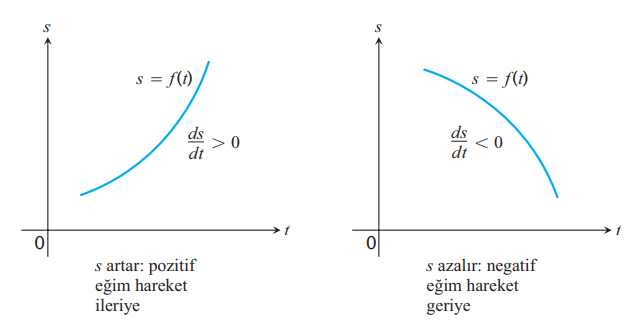
\includegraphics[width=0.7\linewidth]{hizornek.png}
	\caption{Bir doğru boyunca $s=f(t)$ hareketi için $v=ds/dt$, $s$ artarken pozitif, $s$ azalırken negatiftir.}
	\label{fig:ornekresim}
\end{figure}
Bir arkadaşın evine gidip dönerken 30 mil/sa ile gidiyorsak, hız göstergesi giderken 30 mil/sa gösterirken, dönerken, evden uzaklığımız azaldığı halde, -30 mil/sa göstermeyecektir. Hız göstergesi her zaman hızın mutlak değeri olan sürati gösterir. Sürat yönden bağımsız olarak ileri gitme oranını ölçer.
\begin{tanim}
	\textit{Sürat} hızın mutlak değeridir
	\begin{equation*}
	\textit{Sürat} = |v(t)|=\left| \frac{ds}{dt}\right|
	\end{equation*}
\end{tanim}
\begin{ornek}
	Şekil 4.2'de, bir koordinat doğrusu bounca ilerleyen bir parçacığın hızı $v = f'(t)$ görülmektedir. Parçacık ilk 3 saniye boyunca ileri doğru, sonraki 2 saniye boyunca geri doğru hareket etmekte, bir saniye durmakta ve yine ileri doğru hareket etmektedir. Parçacık en yüksek sürate $t=4$ anında, geriye doğru giderken ulaşır.
\begin{figure}[H]
	\centering
	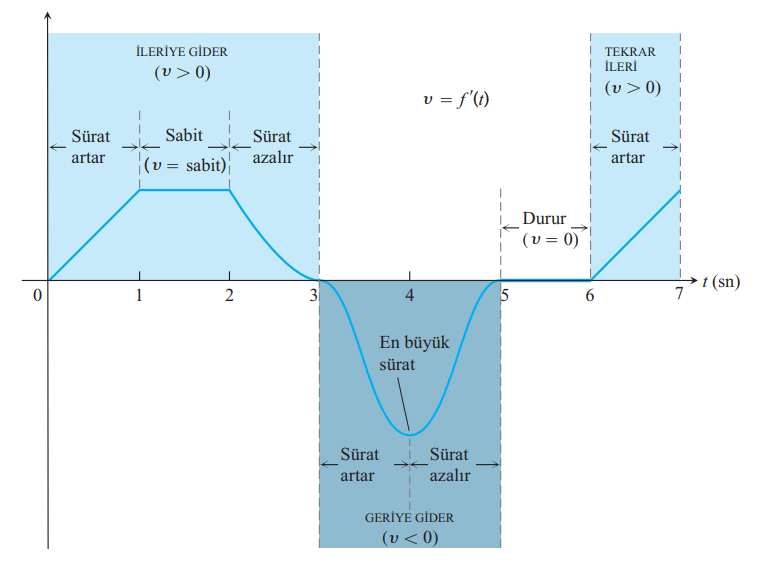
\includegraphics[width=0.7\linewidth]{hizornek2.png}
	\caption{Örnek İçin hız grafiği.}
	\label{fig:ornekresim}
\end{figure}
\end{ornek}
Bir cismin hızının değişim oranına \textit{cismin ivmesi} denir. İvme, bir cismin ne kadar çabuk sürat kazandığını veya kaybettiğini ölçer.\\

İvmedeki ani bir değişime çekme denir. Bir otomobil veya bir otobüsteki yolculuk sarsıntılı olduğunda bu, ilgili ivmelerin mutlaka büyük olmasından değil ivmedeki değişimlerin ani olmasındandır.
\begin{tanim}
	\textit{İvme} hızın zamana göre türevidir. Bir cismin $t$ anındaki konumu $s=f(t)$ ise, cismin $t$ anındaki ivmesi şu şekildedir:
	\begin{equation*}
	a(t)=\frac{dv}{dt}=\frac{d^2 s}{dt^2}
	\end{equation*}
	\textit{Silkinme} ivmenin zamana göre türevidir:
	\begin{equation*}
	j(t)=\frac{da}{dt}=\frac{d^3 s}{dt^3}
	\end{equation*}
\end{tanim}
Dünya yüzeyine yakın yerlerde bütün cisimler aynı sabit ivmeyle düşerler. Galileo'nun serbest düşme ile ilgili deneyi, $s$ mesave ve $g$ de dünyanın yerçekiminden doğan ivme olmak üzere, bizi
	\begin{equation*}
	s=\frac{1}{2}gt^2
	\end{equation*}
denklemine götürür. Bu denklem hava tepkisinin bulunmadığı vakumda geçerlidir, ancak kaya veya çelik aletler gibi yoğun, ağır cisimlerin, havanın tepkisinin onları yavaşlatmaya başlamadığı düşüşünün ilk birkaç saniyesini de çok iyi modeller.\\
	$s =(1/2)gt^2$ denklemindeki $g$'nin değeri $t$ ve $s$'yi ölçmekte kullanılan birimlere bağlıdır. $t$ saniye (standart birim) iken, deniz seviyesindeki ölçümle tanımlanan $g$'nin değeri, İngiliz birimleriyle yaklaşık 32 ft/sn$^2$ (fit bölü saniye kare) ve metrik birimle $g=9.8$ m/sn$^2$(metre bölü saniye kare)d,r. (Bu yerçekimi sabitleri Dünyanın ağırlık merkezinden uzaklığa bağludur ve örneğin Everest teğesinde birazcık daha azdır.)\\
	Sabit olan yer çekimi ivmesinin silkinmesi sıfırdır:
	\begin{equation*}
	j=\frac{d}{dt}(g)=0
	\end{equation*}
Bir cisim serbest düşme sırasında sarsılmaz.

\section{\protect Ekonomide Türevler} \label{bolumetiketi}
Mühendisler \textit{hız} ve \textit{ivme} gibi terimleri hareketi tanımlayan fonksiyonların türevlerini belirtmek için kullanırlar. Ekonomistlerin de değişim oranları ve türevler için özel kelimeleri vardır. Bunlara \textit{marjinaller} derler.\\
	Bir üretim işleminde \textit{üretim maliyeti c(x)} üretilen birim miktarı $x$'in bir fonksiyonudur. \textit{Marjinal üretim maliyeti} ise maliyetin $(c)$ üretim seviyesine $(x)$ göre değişim oranı, dolayısıyla $\frac{dc}{dx}$'tir.\\
	Örneğin, $c(x)$ bir haftada $x$ ton çelik üretmek için gereken dolar miktarı olsun. $x+h$ birim üretmek daha pahalı olacaktır ve $h$  ile bölünmüş maliyet farkı bir haftada ton başına maliyetteki ortalama artıştır:
	\begin{equation*}
	\frac{c(x+h)-c(x)}{h}=\textit{üretilen her h ton fazla çeliğin ortalama maliyeti}
	\end{equation*}
Bu oranın $h \rightarrow 0$ iken limiti, haftalık üretim $x$ ton iken bir haftada daha fazla çelik üretmenin \textit{marjinal maliyetidir}(Şekil 4.3):
\begin{figure}[H]
	\centering
	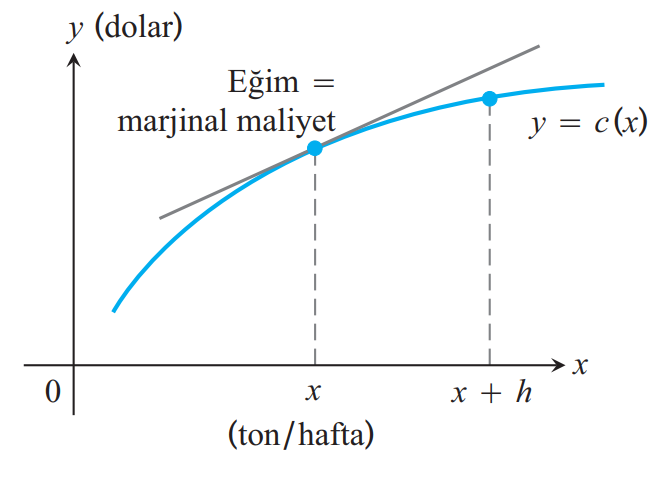
\includegraphics[width=0.5\linewidth]{ekonomideturev1.png}
	\caption{Haftalık çelik üretimi:$c(x)$, haftada $x$ ton üretimin maliyetidir. İlave $h$ ton üretimin maliyeti $c(x+h)-c(x)$dir.}
	\label{fig:ornekresim}
\end{figure}
	\begin{equation*}
	\frac{dc}{dx}=\lim_{h \rightarrow 0}\frac{c(x+h)-c(x)}{h}=\textit{marjinal üretim maliyeti}
	\end{equation*}
Bazen, marjinal üretim maliyeti fazladan bir birim üretmenin maliyeti olarak da tanımlanır:
	\begin{equation*}
	\frac{\varDelta c}{\varDelta x}= \frac{c(x+1)-c(x)}{1}
	\end{equation*}
Bu da yaklaşık olarak $dc/dx$'in $x$'teki değiridir. Bu yaklaşım, $c$'nin grafiği $x$ yakınlarında çok hızlı değişmiyorsa, kabul edilebilirdir. Bu durumda fark bölümü, limitine yani $dc/dx$'e yakın olacaktır, bu da $\varDelta x=1$ is teğetteki yükselmedir(Şekil 4.4). Yaklaşım, büyük $x$ değerlerinde daha iyi sonuç verir.
\begin{figure}[H]
	\centering
	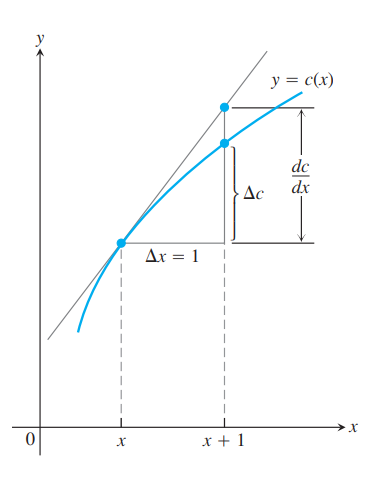
\includegraphics[width=0.5\linewidth]{ekonomideturev2.png}
	\caption{Marjinal maliyet $dc/dx$ üretimin $\varDelta x=1$ birim artmasıyla oluşacak $\varDelta c$ maliyetidir.}
	\label{fig:ornekresim}
\end{figure}
Ekonomistler, toplam maliyet fonksiyonunu genllikle
	\begin{equation*}
	c(x)=\alpha x^3+ \beta x^2 +\gamma x + \delta
	\end{equation*}
Şeklinde bir kübik polinomla temsil ederler. Burada $\gamma$ kira, ısınma, ekipman ve yönetim giderleri gibi \textit{sabit maliyetleri} temsil eder. Diğer terimler hammadde, vergiler ve işçilik gibi \textit{değişken maliyetleri} temsil ederler. Sabit maliyetler üretilen birim sayısından bağımsızdırlar oysa değişken maliyetler üretim miktarına bağlıdırlar. Bir kübik polinom, ilgili nicelik aralığında maliyet davranışını yakalamaya yetecek kadar karmaşıktır.
\begin{ornek}
	8 ile 30 arasında radyatör üretilirken $x$ radyatör üretmenin maliyetinin
	\begin{equation*}
	c(x)=x^3-6x^2+15x
	\end{equation*}
dolar olduğunu ve $x$ radyatör satılmasından elde edilen gelirin
	\begin{equation*}
	r(x)=x^3-3x^2+12x
	\end{equation*}
dolar olduğunu varsayın. Dükkanınız normal olarak günde 10 radyatör üretmektedir. Günde bir radyatör daha üretmek maliyette ne kadar fark edecektir ve günde 11 radyatör satmakla gelirdeki tahmini artış ne olacaktır?
\end{ornek}
\begin{cozum}
Normalde günde 10 radyatör üretilirken, bir radyatör daha fazla üretmenin maliyeti $c'(10)$ civarındadır:
	\begin{equation*}
	\begin{split}
	c'(x)&=\frac{d}{dx}(x^3-6x^2+15x)=3x^2-12x+15\\
	c'(10)&=3(100)-12(10)+15=195
	\end{split}
	\end{equation*}
Ek masraf 195 dolar civarında olacaktır. Marjinal gelir
	\begin{equation*}
	r'(x)=\frac{d}{dx}(x^3-3x^2+12x)=3x^2-6x+12
	\end{equation*}
dir. Marjinal gelir fonksiyonu da fazladan bir birim satıldığında elde edilecek geliri belirtmektedir. Günde 10 radyatör satarken satışınızı 11 radyatöre çıkarırsanız, geliriniz
	\begin{equation*}
	r'(10)=3(100)-6(10)+12=252 \$
	\end{equation*}
kadar artmasını bekleyebilirsiniz.
\end{cozum}
\begin{ornek}
Marjinal oranların diline biraz alışmak için, marjinal vergi oranlarını ele alalım. Marjinal gelir vergisi oranınız \%28 ise ve gelirinizin1000\$ artarsa, gelir vergisi olarak fazladan bir 280\$ vergi vermek zorunda kalacağınızı düşünebilirsiniz. Bu toplam gelirinizin \%28'ini vergi olarak vereceğiniz anlamına gelmez. Sadece şu andaki $I$ gelir düzeyinizde, gelire göre $T$ vergisindeki artış oranının $dT/dI=0.28$ olacağını söyler. Kazandığınız fazladan her dolar için 0.28\$ vergi vereceksinizdir. Elbette kazancınız daha fazla artarsa, vergi diliminiz değişebilir ve marjinal oranınız artabilir.
\end{ornek}
\section{\protect Değişikliğe Duyarlılık} \label{bolumetiketi}
$x$'teki küçük bir değişim bir fonksiyonun değerinde büyük bir değişime yol açtığında, fonksiyonun $x$'teki değişime karşı duyarlı olduğunu söyleriz. $f'(x)$ türevi bu duyarlılığın ölçüsüdür.
\begin{ornek}
Bezelyeler ve başka bitkilerle uğraşan Avusturyalı keşiş Gregor Johann Mendel (1822-1884) melezlemenin ilk bilimsel açıklamalarını ortaya koymuşur.\\
Dikkatlice yapılmış kayıtları, $p$ (0 ile 1 arasında bir sayı) bezelyelerdeki düzgün kabuk geninin (baskın gen) sıklığı ve $(1-p)$ de bezelyelerdeki kıvrık kabuk geninin (çekinik gen) sıklığıysa, düzgün kabuklu bezelyelerin topluluktaki oranının
	\begin{equation*}
	y=2p(1-p)+p^2=2p-p^2
	\end{equation*}
olduğunu göstermiştir. Şekil 4.5a'daki $y-p$ grafiği $y$'nin değerinin, $p$'deki bir değişikliğe, $p$'nin küçük değerleri için, $p$'nin büyük değerleri için olduğundan daha fazla duyarlı olduğunu göstermektedir. Gerçekten de, bu, $p$ 0 civarındayken $dy/dp$'nin 2'ye, $p$ 1 civarındayken de 0'a yakın olduğunu gösteren Şekil 4.5b'deki türev grafiğiyle daha iyi vurgulanmaktadır.
\begin{figure}[H]
	\centering
	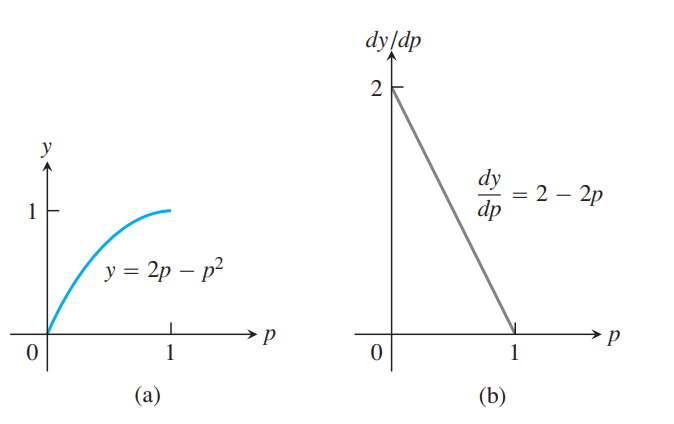
\includegraphics[width=0.7\linewidth]{mendelres.png}
	\caption{(a)Düzgün bezelyelerin oranını belirleyen $y=2p-p^2$ grafiği (b) $dy/dp$ grafiği.}
	\label{fig:ornekresim}
\end{figure}
Genetik için anlamı şudur: Oldukça çekinik bir topluluk içine biraz daha baskın gen eklemek(kıvrık kabuklu bezelye sıklığının az olduğu yerde), oldukça baskın bir topluluktaki benzer artışa göre, sonraki jenerasyonlarda dramatik etkilere neden olacaktır.
\end{ornek}

\chapter{\protect TRİGONOMETRİK FONKSİYONLARIN TÜREVLERİ}
Hakkında bilgi edinmek istediğimiz bir çok olay yaklaşık olarak periyodiktir (elektromanyetik alanlar, kalp atışları, gel-gitler, hava). Sinüslerin ve kosinüslerin türevleri periyodik değişiklikleri tanımlamada anahtar rolü oynarlar. Bu bölüm altı temel trigonametrik fonksiyonun türevlerinin nasıl alınacağını göstermektedir.
\section{\protect Sinüs Fonksiyonunun Türevi} \label{bolumetiketi}
$x$, radyan olarak ölçülmek üzere $f(x) = \sin x$ fonksiyonunun türevini almak için, sinüs için açı toplama özdeşliği ile birleştiririz:
	\begin{equation*}
	\sin (x+h) = \sin x \cos h + \cos x \sin h
	\end{equation*}
$f(x) = \sin x$, ise
	\begin{equation*}
	\begin{split}
		f'(x)&=\lim _{h\rightarrow 0}\dfrac{f\left( x+h\right) -f\left( x\right) }{h}\\
		&=\lim _{h\rightarrow 0}\dfrac{\sin \left( x+h\right) -\sin x}{h}\\
		&=\lim _{h\rightarrow 0}\dfrac{\left( \sin x \cos h +\cos x\sin h \right) -\sin x}{h}\\
		&=\lim _{h\rightarrow 0}\dfrac{\sin x\left( \cos h -1\right) +\cos x\sin h }{h}\\
		&=\lim _{h\rightarrow 0}\left( \sin x\cdot \dfrac{\cos h -1}{h}\right) +\lim _{h\rightarrow 0}\left( \cos x\cdot \dfrac{\sin h }{h}\right)\\
		&=\sin x . \lim_{h \rightarrow 0} \frac{\cos h -1}{h}+\cos x . \lim_{h \rightarrow 0} \frac{\sin h}{h}\\
		&=\sin x . 0 + \cos x . 1\\
		&=\cos x
	\end{split}
	\end{equation*}
Sinüs fonksiyonunun türevi kosinüs fonksiyonudur:
	\begin{equation*}
	\frac{d}{dx}(\sin x) = \cos x
	\end{equation*}
\begin{ornek}Sinüs içeren türevler:\\

	(a)$y = x^2-\sin x:$
	\begin{equation*}
	\begin{split}
		\frac{dy}{dx}&=2x-\frac{d}{dx}(\sin x)\\
		&= 2x - \cos x.
	\end{split}
	\end{equation*}
	(b)$y=x^2\sin x:$
	\begin{equation*}
	\begin{split}
	\frac{dy}{dx}&=x^2\frac{d}{dx}(\sin x) + 2x\sin x\\
	&= x^2\cos x + 2x\sin x.
	\end{split}
	\end{equation*}
	(c)$\displaystyle y= \frac{\sin x}{x}:$
	\begin{equation*}
	\begin{split}
	\frac{dy}{dx}&=\frac{x.\frac{d}{dx}(\sin x)-\sin x . 1}{x^2}\\
	&=\frac{x \cos x - \sin x}{x^2}
	\end{split}
	\end{equation*}
\end{ornek}
\section{\protect Kosinüs Fonksiyonunun Türevi} \label{bolumetiketi}
Kosinüs için
	\begin{equation*}
	\cos(x+h) = \cos x \cos h-\sin x \sin h
	\end{equation*}
açı toplama formülünün yardımıyla,
	\begin{equation*}
	\begin{split}
		\frac{d}{dx}(\cos x)&=	\lim _{h\rightarrow 0}\frac{\cos(x+h)-\cos x}{h}\\
	&=\lim _{h\rightarrow 0}\frac{(\cos x \cos h-\sin x \sin h)-\cos x}{h}\\
	&=\lim _{h\rightarrow 0}\frac{\cos x(\cos h -1)-\sin x\sin h}{h}\\
	&=\lim _{h\rightarrow 0}\cos x.\frac{\cos h -1}{h}-\lim _{h\rightarrow 0}\sin x.\frac{\sin h}{h}\\
	&=\cos x.\lim _{h\rightarrow 0}\frac{\cos h -1}{h}-\sin x.\lim _{h\rightarrow 0}\frac{\sin h}{h}\\
	&=\cos x.0-\sin x.1\\
	&=-\sin x		
	\end{split}
	\end{equation*}
Kosinüs fonksiyonunun türevi sinüs fonksiyonunun negatifidir:
	\begin{equation*}
	\frac{d}{dx}(\cos x)= -\sin x
	\end{equation*}
\begin{ornek}Kosinüs içeren türevler:\\

	(a)$y = 5x+\cos x:$
	\begin{equation*}
	\begin{split}
		\frac{dy}{dx}&=\frac{d}{dx}(5x)+\frac{d}{dx}(\cos x)\\
		&= 5-\sin x.
	\end{split}
	\end{equation*}
	(b)$y=\sin x \cos x:$
	\begin{equation*}
	\begin{split}
	\frac{dy}{dx}&=\sin x \frac{d}{dx}(\cos x)+ \cos x \frac{d}{dx}(\sin x)\\
	&= \sin x(-\sin x)+\cos x(\cos x)\\
	&=\cos^2 x- \sin^2 x
	\end{split}
	\end{equation*}
	(c)$\displaystyle y= \frac{\cos x}{1-\sin x}:$
	\begin{equation*}
	\begin{split}
	\frac{dy}{dx}&= \frac{(1-\sin x)\frac{d}{dx}(\cos x)-\cos x \frac{d}{dx}(1-\sin x)}{(1-\sin x)^2}\\
	&=\frac{(1-\sin x)(-\sin x)-\cos x(0-\cos x)}{(1-\sin x)^2}\\
	&=\frac{1-\sin x}{(1-\sin x)^2}\\
	&= \frac{1}{1-\sin x}
	\end{split}
	\end{equation*}
\end{ornek}
%BURADAN ÖNCESİ ÇALIŞIYOR DOKUNMA%S
\section{\protect Diğer Temel Trigonometrik Fonksiyonların Türevleri} \label{bolumetiketi}
$\sin x$ ve $\cos x$ $x$'in türevlenebilir fonksiyonları oldukları için bunlarla ilişkili
	\begin{equation*}
	\tan x =\frac{\sin x}{\cos x}, \cot x=\frac{\cos x}{\sin x}, \sec x =\frac{1}{\cos x}, \csc x=\frac{1}{\sin x}
	\end{equation*}
fonksiyonları da tanımlı oldukları bütün $x$ değerlerinde türevlenebilirdirler. Bölüm kurallarıyla bulunan türevleri aşağıdaki formüllerle verilir. Kotanjant ve kosekant fonksiyonlarının türev formüllerindeki eksi işaretine dikkat edin.
	\begin{equation*}
	\begin{split}
	\frac{d}{dx}(\tan x)&= \sec^2 x\\
	\frac{d}{dx}(\sec x)&= \sec x\tan x\\
	\frac{d}{dx}(\cot x)&= -\csc^2 x\\
	\frac{d}{dx}(\csc x)&=- \csc x\cot x
	\end{split}
	\end{equation*}

\begin{ornek}$d(\tan x)/dx$'i bulun.
\end{ornek}
\begin{cozum}
	\begin{equation*}
	\begin{split}
	\dfrac{d}{dx}\left( \tan x\right) &=\dfrac{d}{dx}\left( \dfrac{\sin x}{\cos x}\right) =\dfrac{\cos x\dfrac{d}{dx}\left( \sin x\right) -\sin x\dfrac{d}{dx}\left( \cos x\right) }{\cos ^{2}x}\\
	&=\dfrac{cosx\cos x-\sin x\left( -\sin x\right) }{\cos ^{2}x}\\
	&=\dfrac{cos^{2}x+\sin ^{2}x}{\cos ^{2}x}\\
	&=\dfrac{1}{\cos ^{2}x}=\sec ^{2}x
	\end{split}
	\end{equation*}
\end{cozum}
\\


\begin{ornek}$y=\sec x$ ise $y''$'nü bulun.
\end{ornek}
\begin{cozum}
	\begin{equation*}
	\begin{split}
	y&=\sec x\\
	y'&=\sec x \tan x \\
	y''&=\frac{d}{dx}(\sec x \tan x)\\
	&=\sec x\frac{d}{dx}(\tan x)+\tan x\frac{d}{dx}(\sec x)\\
	&=\sec x(\sec ^2 x)+\tan x(\sec x \tan x)\\
	&=\sec ^3 x + \sec x \tan ^2 x
	\end{split}
	\end{equation*}
\end{cozum}


Trigonometrik fonksiyonların, tanım kümelerinin tamamında türevlenebilir olmaları, tanım kümelerinin her noktasında sürekliliklerinin bir başka ispatıdır(bkz. Teorem 2.8.1). Dolayısıyla, trigonometrik fonksiyonların cebirsel kombinasyonlarının ve bileşkelerinin limitlerini doğrudan yerine yazma ile hesaplayabiliriz.
\begin{ornek}Bir trigonometrik limit bulma
	\begin{equation*}
	\lim_{x \rightarrow 0}\frac{\sqrt{2+\sec x}}{\cos (\pi - \tan x)}=\frac{\sqrt{2+\sec 0}}{\cos (\pi - \tan 0)}=\frac{\sqrt{2+1}}{\cos (\pi - 0)}=\frac{\sqrt{3}}{-1}=-\sqrt{3}
	\end{equation*}
\end{ornek}

\chapter{\protect ZİNCİR KURALI ve PARAMETRİK DENKLEMLER}
$y=f(u)=\sin u$ ve $u=g(x)=x^2-4$ fonksiyonlarının türevlerini nasıl alacağımızı biliyoruz, fakat $F(x)=f(g(x))=\sin (x^2-4)$ gibi bir bileşkenin türevini nasıl alırız? Yani $F(x) = f \circ g$'nin türevini nasıl buluruz? Cevap, iki türevlenebilir fonksiyonun bileşkesinin türevinin, iki fonksiyonun da uygun noktalarda alınmış türevlerinin çarpımı olduğunu söyleyen zincir kuralıdır. Zincir kuralı büyük olasılıkla matematikte en sık kullanılan türev alma yöntemidir. Bu bölüm, kuralı ve nasıl kullanılacağını tanımlamaktadır.
\section{\protect Bir Bileşke Fonksiyonun Türevi}
\begin{ornek}Türevleri İlişkilendirmek\\
	$\displaystyle y=\frac{3}{2}x=\frac{1}{2}(3x)$ fonksiyonu $y=\frac{1}{2}u$ ve $u=3x$ fonksiyonlarının bileşkesidir. Bu üç fonksiyonun türevlerinin arasındaki ilişki nedir?
\end{ornek}
\begin{cozum}
	\begin{equation*}
	\frac{dy}{dx}=\frac{3}{2}, \frac{dy}{du}=\frac{1}{2} \textit{  ve  } \frac{du}{dx}=3
	\end{equation*}
olduğunu biliyoruz. $\displaystyle \frac{3}{2}=\frac{1}{2}.3$ olduğundan,
	\begin{equation*}
	\frac{dy}{dx}=\frac{dy}{du}.\frac{du}{dx}
	\end{equation*}
buluruz.
	\begin{equation*}
	\frac{dy}{dx}=\frac{dy}{du}.\frac{du}{dx}
	\end{equation*}
olması bir tesadüf müdür? Türevi bir değişim oranı olarak düşünürsek, şimdiye kadar öğrendiklerimiz bu ilişkinin mantıklı olduğunu gösterir.$y=f(u)$ ve $u=g(x)$ için, $y$ $u$'nun yarısı kadar hızlı değişiyor ve $u$ da $x$'in üç katı kadar hızlı değişiyorsa, $y$'nin $x$'in 3/2 katı hızlı değişmesini bekleriz. 
\end{cozum}
\begin{ornek}
	\begin{equation*}
	y=9x^4+6x^2+1=(3x^2+1)^2
	\end{equation*}
$y=u^2$ ve $u=3x^2+1$ fonksiyonlarının bileşkesidir. Türevleri hesaplarsak,
	\begin{equation*}
	\begin{split}
	\frac{dy}{du}.\frac{du}{dx}&=2u.6x\\
	&=2(3x^2+1).6x\\
	&=36x^3+12x
	\end{split}
	\end{equation*}
olduğunu görürüz. Türevleri açık formülden hesaplarsak
	\begin{equation*}
	\begin{split}
	\frac{dy}{dx}&=\frac{d}{dx}(9x^4+6x^2+1)\\
		&=36x^3+12x
	\end{split}
	\end{equation*}
elde ederiz. Bir kere daha
	\begin{equation*}
	\frac{dy}{du}.\frac{du}{dx}=\frac{dy}{dx}
	\end{equation*}
ile karşılaşırız.
\end{ornek}

$f(g(x))$ bileşke fonksiyonunun $x$'teki türevi $f$'nin $g(x)$'teki türevi çarpı $g$'nin $x$'teki türevidir. Buna zincir kuralı denir(Şekil 6.1).
\begin{figure}[H]
	\centering
	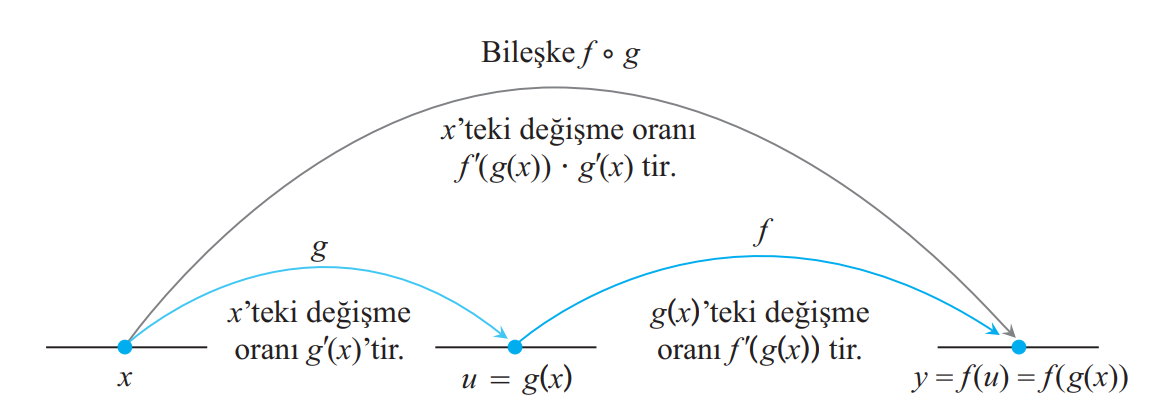
\includegraphics[width=1\linewidth]{bilesketurev.png}
	\caption{Değişim oranları çarpılır: $f \circ g$'nin $x$'teki türevi $f$'nin $g(x)$ noktasındaki türevi çarpı $g$'nin $x$'teki türevidir.}
	\label{fig:ornekresim}
\end{figure}

\begin{teorem} \textit{Zincir Kuralı:}\\
$f(u)$ $u=g(x)$ noktasında türevlenebiliyorsa ve $g(x)$ de $x$'te türevlenebiliyorsa $(f \circ g)(x)=f(g(x))$ bileşke fonksiyonu da $x$'te türevelenebilir ve bu türev
	\begin{equation*}
	(f \circ g)'(x)=f'(g(x)).g'(x)
	\end{equation*}
olur. Leibnitz gösterimiyle, $y=f(u)$ ve $u=g(x)$ ise, bu
	\begin{equation*}
	\frac{dy}{dx}=\frac{dy}{du}.\frac{du}{dx}
	\end{equation*}
olarak yazılır. Burada $dy/du$ $u=g(x)$'te hesaplanmaktadır.
\end{teorem}
\begin{ispat}
	\textit{Zincir Kuralının Sezgisel "İspatı":}\\
$x$'teki $\varDelta x$ değişimine karşılık $u$'daki değişme $\varDelta u$ olsun, yani
	\begin{equation*}
	\varDelta u=g(x+\varDelta x)-g(x)
	\end{equation*}
olsun. Buna karşılık $y$'deki değişme
	\begin{equation*}
	\varDelta y=f(u+\varDelta u)-f(u)
	\end{equation*}
olur.
	\begin{equation}
	\frac{\varDelta y}{\varDelta x} = \frac{\varDelta y}{\varDelta u}.\frac{\varDelta u}{\varDelta x}
	\end{equation}
yazmak ve $\varDelta x \rightarrow 0$ iken limitini almak ilginç olabilir:
	\begin{equation*}
	\begin{split}
	\frac{dy}{dx}&=\lim_{\varDelta x \rightarrow 0}\frac{\varDelta y}{\varDelta x}\\
		&=\lim_{\varDelta x \rightarrow 0}\frac{\varDelta y}{\varDelta u}.\frac{\varDelta u}{\varDelta x}\\
		&=\lim_{\varDelta x \rightarrow 0}\frac{\varDelta y}{\varDelta u}.\lim_{\varDelta x \rightarrow 0}\frac{\varDelta u}{\varDelta x}\\
		&=\lim_{\varDelta u \rightarrow 0}\frac{\varDelta y}{\varDelta u}.\lim_{\varDelta x \rightarrow 0}\frac{\varDelta u}{\varDelta x}\\
		&=\frac{dy}{dx}\frac{du}{dx}
	\end{split}
	\end{equation*}
Bu akıl yürütmedeki tek pürüz (6.1) denkleminde $\varDelta u = 0$ olabilir ($\varDelta u $$\ne$$ 0$ olduğu halde) ve şüphesiz ki 0 ile bölemeyiz. İspat, bu pürüzün üstesinden gelmek için farklı bir yaklaşım gerektirmektedir ve "Lineerizasyon ve Diferansiyeller" konusunda tam ispatını vereceğiz.
\end{ispat}

\begin{ornek}\textit{Zincir Kuralını Uygulamak}
$x$-ekseni üzerinde hareket eden bir cismin her $t \geq 0$ zamanındaki konumu $x(t)=\cos (t^2+1)$ ile veriliyor. Cismin hızını, $t$'nin bir fonksiyonu olarak bulun.
\end{ornek}
\begin{cozum}
	Hızın $dx/dt$ olduğunu biliyoruz. Bu arada, $x$ bir bileşke fonksiyondur: $x=\cos (u)$ ve $u=t^2+1$.
	\begin{equation*}
	\begin{split}
	\frac{dx}{du}&=-\sin (u)\\
	\frac{du}{dt}=2t
	\end{split}
	\end{equation*}
buluruz. Zincir kuralına göre,
	\begin{equation*}
	\begin{split}
	\frac{dx}{dt}&=\frac{dx}{du}.\frac{dx}{dt}\\
		&=-\sin (u).2t\\
		&=-\sin (t^2+1).2t\\
		&=-2t\sin(t^2+1)
	\end{split}
	\end{equation*}
bulunur.
\end{cozum}
\section{\protect "İç-Dış" Kuralı}
Bazen zincir kuralını şu şekilde düşünmek yararlı olabilir: $y=f(g(x))$ ise
	\begin{equation*}
		\frac{dy}{dx}=f'(g(x)).g'(x)
	\end{equation*}
dir. Yani, "dış" fonksiyon $f$'in türevini alın ve "iç" fonksiyon $g(x)$'e dokunmayın; sonra da iç fonksiyon $g(x)$'in türeviyle çarpın.
\begin{ornek}\textit{Dıştan İçe Türev Almak}\\
$\sin (x^2+x)$'in $x$'e göre türevini alın.
\end{ornek}
\begin{cozum}
	\begin{equation*}
	\frac{d}{dx}\sin (x^2+x)=\cos (x^2+x).(2x+1)
	\end{equation*}
\end{cozum}
\section{\protect Zincir Kuralının Üst Üste Kullanılması}
Bazen bir türevi bulabilmek için zincir kuralını iki veya daha fazla defa kullanmamız gerekebilir. Aşağıda buna bir örnek verilmektedir.
\begin{ornek}\textit{Üç Halkalı Bir "Zincir"}\\
$g(t)=\tan (5-\sin{2t})$ fonksiyonunun türevini bulun.
\end{ornek}
\begin{cozum} Burada şuna dikkat edin, teğet $5-\sin{2t}$'nin fonksiyonudur. Oysa sinüs fonksiyonu, kendisi de $t$'nin bir fonksiyonu olan $2t$'nin fonksiyonudur. Bu nedenle Zincir Kuralı'ndan
	\begin{equation*}
	\begin{split}
	g'(t)&=\frac{d}{dt}(\tan (5-\sin{2t}))\\
		&=\sec ^2(5-\sin{2t}).\frac{d}{dt}(5-\sin{2t})\\
		&=\sec ^2(5-\sin{2t}).\left(0-\cos{2t}.\frac{d}{dt}(2t)\right)\\
		&=\sec ^2(5-\sin{2t}).(-\cos {2t}).2\\
		&=-2(\cos{2t}\sec ^2(5-\sin{2t})
	\end{split}
	\end{equation*}
elde edilir.
\end{cozum}
\section{\protect Zincir Kuralı ve Bir Fonksiyonun Kuvveti}
$f$, $u$'nun türevlenebilir bir fonksiyonu ve $u$ da $x$'in türevlenebilir bir fonksiyonu ise,
	\begin{equation*}
	\frac{dy}{dx}=\frac{dy}{du}.\frac{du}{dx}
	\end{equation*}
zincir kuralından $y=f(u)$ yazmak
	\begin{equation*}
	\frac{d}{dx}f(u)=f'(u)\frac{du}{dx}
	\end{equation*}
formülüne götürür.\\
	Nasıl çalıştığına dair bir örnek aşağıdadır: $n$ bir tamsayıysa, pozitif veya negatif, ve $f(u)=u^n$ ise, Kuvvet Kuralı $f'(u)=nu^{n-1}$ olduğunu söyler. $u$, $x$'in türevlenebilir bir fonksiyonu ise bunu, Zincir Kuralını \textit{Kuvvet Zincir Kuralı}'na genişletmek için kullanabiliriz:
	\begin{equation*}
	\frac{d}{dx}u^n=nu^{n-1}\frac{du}{dx}
	\end{equation*}\\


\begin{ornek}\textit{Kuvvet Zincir Kuralını Uygulamak}\\
(a)\begin{equation*}
	\begin{split}
	\frac{d}{dx}(5x^3-x^4)^7&=7(5x^3-x^4)^6\frac{d}{dx}(5x^3-x^4)\\
		&=7(5x^3-x^4)^6(5.3x^2-4x^3)\\
		&=7(5x^3-x^4)^6(15x^2-4x^3)
	\end{split}
	\end{equation*}
(b)\begin{equation*}
	\begin{split}
	\frac{d}{dx}\left(\frac{1}{3x-2}\right)&=\frac{d}{dx}(3x-2)^{-1}\\
		&=-1(3x-2)^{-2}\frac{d}{dx}(3x-2)\\
		&=-1(3x-2)^{-2}(3)\\
		&=-\frac{3}{(3x-2)^2}
	\end{split}
	\end{equation*}
\end{ornek}
\begin{ornek}\textit{Radyan ve derece}\\
$\sin x$ ve $\cos x$'in türev formüllerinin $x$'in derece değil, radyan olarak ölçüldüğü varsayımı altında çıkarıldığını unutmamak çok önemlidir. Zincir kuralı bu ikisi arasındaki farkı anlamaya daha iyi yardımcı olur. $180^{\circ}=\pi$ radyan olduğu için, $x^{\circ}=\pi x/180$ radyan olur.\\
Zincir kuralını kullanarak
	\begin{equation*}
	\frac{d}{dx}\sin(x^{\circ})=\frac{d}{dx}\sin \left(\frac{\pi x}{180}\right) =\frac{\pi}{180}\cos \left( \frac{\pi x}{180} \right)=\frac{\pi}{180}\cos (x^{\circ})
	\end{equation*}
buluruz. Şekil 6.2 bakın. Aynı şekilde, $\cos (x^{\circ})$'in türevi $-(\pi / 180)\sin(x^{\circ})$ olur.\\
Daha ilk türevde rahatsız edici görünen $\pi /180$ faktörünü üst üste türev almayla daha da belirginleşecektir. Bir bakışta radyan ölçü kullanmanın neden daha çekici olduğu anlaşılmaktadır.
\begin{figure}[H]
	\centering
	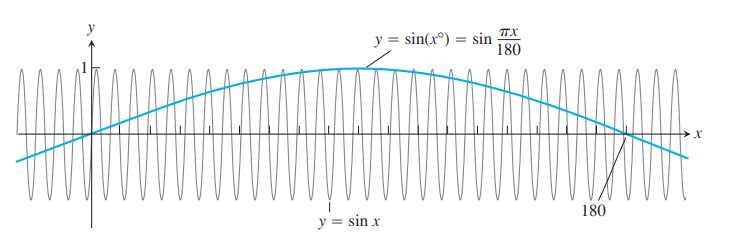
\includegraphics[width=0.8\linewidth]{sinusradyan.png}
	\caption{$\sin x$'in salınmasına karşın $\sin(x^{\circ})$ sadece $\pi / 180$ defa fazla salınır.Maksimum  eğim, $x=0$ da $\pi /180$'dir.}
	\label{fig:ornekresim}
\end{figure}
\end{ornek}
\section{\protect Parametrik Denklemler}
Bir eğriyi eğri üzerindeki bir $P(x,y)$ noktasının $y$- koordinatını $x$'in bir fonksiyonu olarak ifade etmekle tanımlamak yerine, bazen her iki koordinatı da bir üçüncü değişken $t$ cinsinden ifade etmek daha uygundur. Şekil 6.3 de bir cismin, bir çift denklem $x=f(t)$, $y=g(t)$, ile tanımlı yolu görülmektedir. Hareket incelemesinde $t$ genellikle zamanı gösterir. Bu gibi denklemler, herhangi bir $t$ anında parçacığın $(x,y)=(f(t),g(t))$ konumunu verdikleri için bir kartezyen formülden daha iyidirler.

\begin{figure}[H]
	\centering
	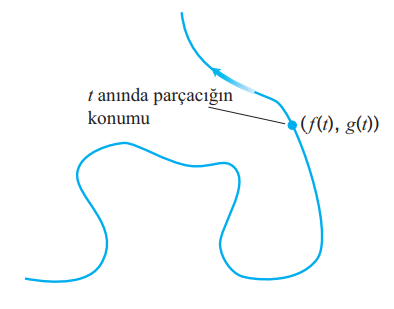
\includegraphics[width=0.4\linewidth]{parametrik1.png}
	\caption{$xy$- düzleminde ilerleyen bir parçacığın izlediği yol her zaman $x$'in veya $y$'nin bir fonksiyonun grafiği değildir.}
	\label{fig:ornekresim}
\end{figure}
\begin{tanim}\textit{Parametrik Eğri}\\
	$x$ ve $y$, bir $t$ değerleri aralığında
	\begin{equation*}
	x=f(t),	y=g(t)
	\end{equation*}
fonksiyonları olarak verilmişse, bu denklemlerle tanımlanan $(x,y)=(f(t),g(t))$ noktalarının kümesi \textit{bir parametrik eğridir}. Denklemler, eğrinin \textit{parametrik denklemleridir}.
\end{tanim}

$t$ değişkeni eğrinin bir parametresi ve tanım kümesi $I$, \textit{parametre aralığıdır}. $I$ kapalı aralıksa, $a \leq t \leq b$, $(f(a),g(a))$ noktası eğrinin başlangıç noktası ve $(f(b),g(b))$noktası eğrinin bitiş noktasıdır. Düzlemdeki bir eğri için parametrik denklemleri ve parametre aralığını verirsek, eğriyi \textit{parametrize} ettiğimizi söyleriz. Denklemler ve aralık eğrinin \textit{parametrizasyonunu} verir.
\begin{ornek}\textit{Bir Çember Üzerinde Saat Yönünün Tersine Hareket}\\
Aşağıdaki parametrik eğrilerin grafiklerini çizin.\\
(a)$x= \cos t$,		$y= \sin t$,		$0 \leq t \leq 2\pi$.
(b)$x= a\cos t$,		$y= a\sin t$,		$0 \leq t \leq 2\pi$.
\end{ornek}
\begin{figure}[H]
	\centering
	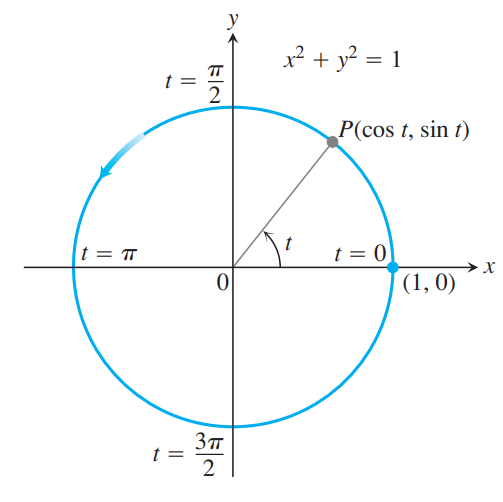
\includegraphics[width=0.4\linewidth]{parametrik2.png}
	\caption{$x=\cos t$, $y= \sin t$ denklemleri $ x^2+y^2=1$ çemberi üzerindeki hareketi tanımlarlar. Ok artan $t$ yönünü göstermektedir.(Örnek 6.5.1)}
	\label{fig:ornekresim}
\end{figure}
\begin{cozum}\\
(a) $x^2+y^2 = \cos ^2 t+ \sin	^2 t = 1$ olduğundan, parametrik eğri $x^2+y^2 =1$ çemberi üzerindedir. $t$ 0'dan $2\pi$'ye artarken $(x,y)=(\cos t, \sin t)$ noktası $(1,0)$'dan başlar ve saat yönünün tersine olarak bütün çemberi çizer (Şekil 6.4).\\
(b) $x= a \cos t$, $y= a \sin t$, $0 \leq t \leq 2\pi$ için $x^2+y^2 =a^2 \cos ^2 t+ a^2 \sin ^2 t=a^2$dir. Parametrizasyon, $(a,0)$ başlayıp $x^2+y^2=a^2$ çemberini saat yönünün tersine bir defa kat eden ve $t=2\pi$'de $(a,0)$ noktasına dönen hareketi tanımlar.
\end{cozum}

\begin{ornek}\textit{Bir Parabol Boyunca Hareket}\\
$xy$-düzleminde ilerleyen bir parçacığın $P(x,y)$ konumu 
	\begin{equation*}
	x=\sqrt{t},\textit{       		}	y=t,	\textit{       		} t\geq0
	\end{equation*}
denklemleri ve parametre aralığıyla verilmektedir. Parçacığın izlediği yolu belirleyin ve hareketi tanımlayın.
\end{ornek}
\begin{cozum} İzlenen yolu $x =\sqrt{t}$ ve $y=t$ denklemleri arasında $t$'yi yok ederek bulmaya çalışırız. Şansımız varsa, bu $x$ ve $y$ arasında tanımlanabilir bir cebirsel bağıntı verecektir. Bu şekilde
	\begin{equation*}
	y=t=(\sqrt{t})^2=x=2
	\end{equation*}
buluruz. Bu, parçacığın konum koordinatlarının $y=x^2$ denklemini sağladığını gösterir, dolayısıyla parçacık $y=x^2$ parabolü boyunca hareket eder.\\
	Ancak parçacığın izlediği yolun tüm $y=x^2$ parabolü olduğunu düşünmek bir hatadır---bu yol parabolün sadece yarısıdır. Parçacığın $x$ koordinatı hiçbir zaman negatif değildir. Parçacık $t=0$ iken (0,0)'dan harekete başlar ve $t$ arttıkça birinci dörtte bir bölgede yükselir.(Şekil 6.5). Parametre aralığı $[0,\infty)$ dur ve bir bitiş noktası yoktur.
\begin{figure}[H]
	\centering
	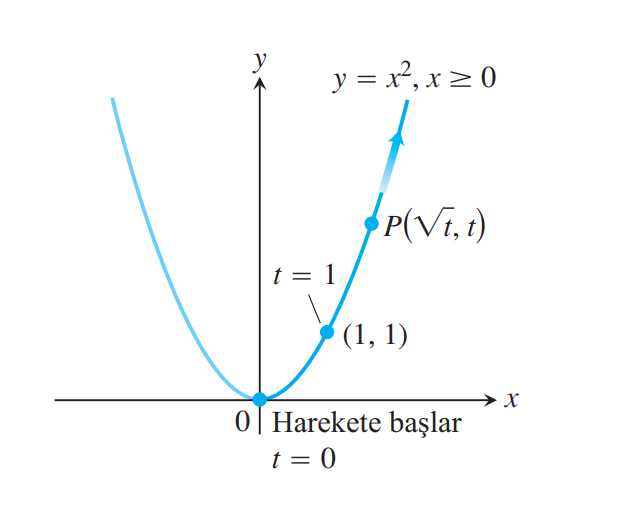
\includegraphics[width=0.4\linewidth]{parametrik3.png}
	\caption{$x=\sqrt{t}$ ve $y=t$ denklemleri ve $ t\geq0$ aralığı, $y=x^2$ parabolünün sağ kolunda ilerleyen bir parçacığın hareketini tanımlar(Örnek 6.5.2).}
	\label{fig:ornekresim}
\end{figure}
\end{cozum}\\


\section{\protect Parametrize Eğrilerin Eğimleri } \label{bolumetiketi}
$f$ ve $g$ fonksiyonları $t$'de türevlenebiliyorsa, parametrize $x=f(t), y=g(t)$ eğrisi de $t$'de \textit{türevlenebilirdir}, $y$'nin de $x$'in sürekli bir fonksiyonu olduğu türevlenebilir parametrize bir eğrinin üzerindeki bir noktada $dy/dt, dx/dt$ ve $dy/dx$ türevleri Zincir Kuralı'na göre bağlıdırlar:
	\begin{equation*}
	\frac{dy}{dt}=\frac{dy}{dx}.\frac{dx}{dt}
	\end{equation*}
$dx/dt \ne 0$ ise, denklemin iki tarafını da $dx/dt$ ile bölerek, $dy/dx$'i çözebiliriz.\\
\subsection{\protect $dy/dx$ İçin Parametrik Formül}
Her üç türev varsa ve $dx/dt \ne 0$ ise
	\begin{equation}
	\frac{dy}{dx}=\frac{dy/dt}{dx/dt}
\end{equation}
dir.
\begin{ornek}\textit{Parametre ile Türetmek}\\
$x=2t +3$ ve $y=t^2-1$ ise $dy/dx$'in $t=6$'daki değerini bulun.
\end{ornek}
\begin{cozum}
(6.2) denklemi $dy/dx$'i $t$'nin bir fonksiyonu olarak verir
	\begin{equation*}
	\frac{dy}{dx}= \frac{dy/dt}{dx/dt}=\frac{2t}{2}=t=\frac{x-3}{2}
	\end{equation*}
$t=6$ için $dy/dx =6 $ olur. Şuna dikkat edin, $dy/dx$ türevini $x$'in bir fonksiyonu olarak da bulabiliriz.
\end{cozum}
\begin{ornek} $x^2/a^2 +y^2/b^2 =1$ \textit{Elipsi Boyunca Hareket}\\
$t$ anındaki konumu $P(x,y)$ 
	\begin{equation*}
	x=a \cos t ,\textit{ 	} y= b \sin t , \textit{ 		} 0 \leq t \leq 2\pi
	\end{equation*}
ile verilen bir parçacığın hareketini tanımlayın, $t =\pi/ 4$ olduğu $(a/\sqrt{2},b/\sqrt{2})$, noktasında eğriye teğet olan doğruyu bulun ($a$ ve $b$ sabitlerinin her ikisi de pozitiftir).
\end{ornek}
\begin{cozum}
	\begin{equation*}
	\cos t= \frac{x}{a},\textit{ 		} \sin t= \frac{y}{b}
	\end{equation*}
denklemlerinden $t$'yi yok ederek, parçacığın konumu için bir Kartezyen denklem buluruz. Bunu $\cos^2t+\sin^2t =1$ bağıntısını kullanarak yaparız. Bu bağıntı
	\begin{equation*}
	\left( \dfrac{x}{a}\right) ^{2}+\left( \dfrac{y}{b}\right) ^{2}=1,\textit{ 	veya	} \frac{x^2}{a^2}+\frac{y^2}{b^2}=1
	\end{equation*}
verir. Parçacığın $(x,y)$ koordinatları $(x^2/a^2)+(y^2/b^2)=1$ denklemini sağlar, dolayısıyla parçacık bu elips üzerinde hareket eder. $t=0$ iken parçacığın koordinatları
	\begin{equation*}
	x=a \cos (0) =a  \textit{, 	} y= b \sin (0) = 0
	\end{equation*}
olur, dolayısıyla hareket $(a,0)$'da başlar. $t$ artarken, parçacık yükselir ve saat yönünün tersine sola doğru hareket eder. Elipsi bir kere dolaşarak $t=2\pi$ iken başlangıç noktası $(a,0)$'a döner.\\
	$t= \pi /4$ için elipse teğet olan doğrunun eğimi
	\begin{equation*}
	\begin{split}
	\frac{dy}{dx}|_{t=\pi/4} &=\frac{dy/dt}{dx/dt}|_{t=\pi/4} 	\textit{ 		 Denklem(6.2)}\\
	&=\frac{b \cos t}{-a \sin t}|_{t=\pi/4}\\
	&=\frac{b/\sqrt{2}}{-a/\sqrt{2}}=-\frac{b}{a}
		\end{split}
	\end{equation*}
dir.\\
Teğet doğru
	\begin{equation*}
	\begin{split}
	y-\frac{b}{\sqrt{2}}&=-\frac{b}{a}\left( x-\frac{a}{\sqrt{2}}\right)\\
	y&=\frac{b}{\sqrt{2}}-\frac{b}{a}\left(x-\frac{a}{\sqrt{2}}\right)
	\end{split}
	\end{equation*}
veya	
	\begin{equation*}
	y= -\frac{b}{a}x+ \sqrt{2}b
	\end{equation*}
\end{cozum}
	Parametrik denklemler $y$'yi $x$'in iki kere türevlenebilir bir fonksiyonu olarak tanımlıyorsa, $d^2y/dx^2$'yi $t$'nin bir fonksiyonu olarak hesaplamak için  \textit{Denklem(6.2)} yi $dy/dx=y'$'ye uygulayabiliriz:
	\begin{equation*}
	\frac{d^2y}{dx^2}=\frac{d}{dx}(y') = \frac{dy'/dt}{dx/dt}.\textit{(Denklem(6.2)de y yerine y' yazılmış.)}
	\end{equation*}\\

\subsection{\protect $d^2y/dx^2$ İçin Parametrik Formül}
$x=f(t)$, $y=g(t)$ denklemleri $y$'yi $x$'in iki kere türevlenebilir bir fonksiyonu olarak tanımlanıyors, $dx/dt$ $\ne$ $0$ olan her noktada
	\begin{equation}
	\frac{d^2y}{dx^2}=\frac{dy'/dt}{dx/dt}
	\end{equation}
\begin{ornek}\textit{Parametrize Bir Eğri İçin} $d^2y/dx^2$'yi Bulmak\\
$x=t-t^2$ ve $y=t-t^3$ ise $d^2y/dx^2$'yi bulun.
\end{ornek}
\begin{cozum}
1. $y' =dy/dx$'i $t$ cinsinden ifade edin:
	\begin{equation*}
	y'=\frac{dy}{dx}=\frac{dy/dt}{dx/dt}=\frac{1-3t^2}{1-2t}
	\end{equation*}
2. $y'$'nün $t$'ye göre türevini alın:
	\begin{equation*}
	\frac{dy'}{dt}=\frac{dy'/dt}{dx/dt}=\frac{(2-6t+6t^2)/(1-2t)^2}{1-2t}=\frac{2-6t+6t^2}{(1-2t)^3}\textit{(Denklem(6.3)ten}
	\end{equation*}
\end{cozum}\\


\subsection{\protect Standart Parametrizasyonlar ve Türev Kuralları}
\textit{ÇEMBER}  $x^2+y^2=1$:
	\begin{equation*}
	\begin{split}
	x&=a \cos t\\
	y&=b \sin t\\
	0 &\leq t \leq 2\pi
	\end{split}
	\end{equation*}
\textit{ELİPS}  $\displaystyle \frac{x^2}{a^2}+\frac{y^2}{b^2}=1$:
	\begin{equation*}
	\begin{split}
	x&=a \cos t\\
	y&=b \sin t\\
	0 &\leq t \leq 2\pi
	\end{split}
	\end{equation*}
\textit{FONKSİYON} $y=f(x)$:
	\begin{equation*}
	\begin{split}
	x&=t\\
	y&=f(t)
	\end{split}
	\end{equation*}
\textit{TÜREVLER} 
	\begin{equation*}
	\begin{split}
	y'=\frac{dy}{dx}&=\frac{dy/dt}{dx/dt}\\
	y''=\frac{d^2y}{dx^2}&=\frac{dy'/dt}{dx/dt}
	\end{split}
	\end{equation*}

\chapter{\protect KAPALI TÜREV ALMA}
Şimdiye kadar ilgilendiğimiz fonksiyonların bir çoğu $y$yi $x$ değişkeni cinsinden açıkça ifade eden $y=f(x)$ şeklindeki bir denklemle tanımlamıştı. Bu şekilde tanımlanan fonksiyonların türevlerini almak için kurallar öğrendik. Bölüm 6'da ayrıca, bir eğri $x=x(t)$ ve $y=y(t)$ denklemleriyle parametrik olarak tanımlandığında $dy/dx$ türevinin nasıl bulunacağını öğrendik. Üçüncü bir durum
	\begin{equation*}
	x^2+y^2-25=0 \textit{    ,   } y^2-x=0 \textit{    veya  }  x^3+y^3-9xy=0
	\end{equation*}
şeklinde denklemlerle karşılaştığımızda ortaya çıkar(bkz. Şekil 7.2 ve 7.3). Bu denklemler $x$ ve $y$ değişkenleri arasında kapalı bir bağıntı tanılmlarlar. Bazı durumlarda böyle bir denklemden $y$'yi $x$'in açık fonksiyonu olarak (veya belki birkaç fonksiyon) çözebiliriz. Bir $F(x,y)=0$ denklemini bildiğimiz şekilde türevini alabilmek için $y=f(x)$ haline sokamadığımızda, kapalı türev alma yöntemiyle $dy/dx$'i yine de bulabiliriz. Bu, denklemin her iki tarafının da $x$'e göre türevini almaktan ve sonra sonuç denklemi $y'$'ye göre çözmekten ibarettir. Bu bölümde bu yöntem anlatılmakta ve bu yöntem kullanılarak kuvvet kuralı, tüm rasyonel üsleri kapsayacak şekilde genişletilmektedir. Bu bölümdeki örneklerde verilen denklemlerin, daima $y$'yi ve $x$'in türevlenebilir bir fonksiyonu olarak tanımladıkları kabul edilmektedir.

\begin{figure}[H]
	\centering
	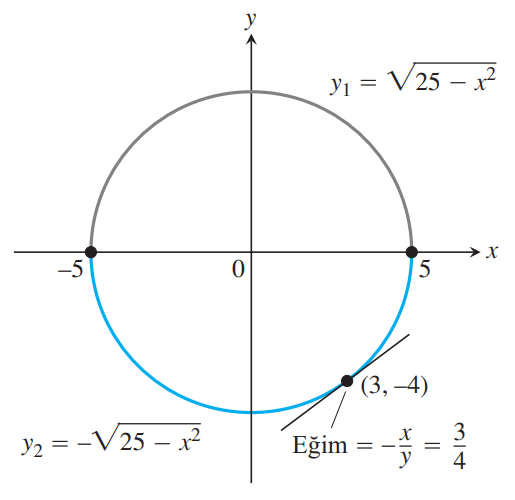
\includegraphics[width=0.5\linewidth]{kapaliturev1.png}
	\caption{Çember iki fonksiyonun grafiklerini birleştirir. $y_2$ grafiği alt yarı çemberdir ve (3,-4) noktasından geçer.}
	\label{fig:ornekresim}
\end{figure}
\section{\protect Kapalı Olarak Tanımlı Fonksiyonlar}
\begin{ornek}\textit{Kapalı Olarak Türev Alma}\\
	$y^2=x$ ise $dy/dx$'i bulun.
\end{ornek}
\begin{cozum}
	$y^2=x$ denklemi $x$'in türevlenebilir ve aslında bulabileceğimiz iki fonksiyonunu tanımlar, yani $y_1=\sqrt{x}$ ve $y_2=-\sqrt{x}$ (Şekil 7.2). İkisinin de $x>0$ türevlerinin nasıl alınacağını biliyoruz:
	\begin{equation*}
	\frac{dy_1}{dx}=\frac{1}{2\sqrt{x}} \textit{ve} \frac{dy_2}{dx}=-\frac{1}{2\sqrt{x}}
	\end{equation*}
Ama sadece $y^2=x$ denklemini sağlayan $y$'yi $x>0$ için $x$'in bir veya daha fazla türevlenebilir fonksiyonu olarak tanımladığını bildiğimizi varsayalım (açık olarak bilmesek de). Hala $dy/dx$'i bulabilir miyiz?\\
Yanıt evettir. $dy/dx$'i bulmak için, $y=f(x)$'e $x$'in türevlenebilir bir fonksiyonuymuş gibi davranarak, $y^2=x$ denkleminin iki tarafının da $x$'e göre türevini alırız:
	\begin{equation*}
	\begin{split}
	y^2&=x\\
	2y	\frac{dy}{dx}&=1\\
	\frac{dy}{dx}&=\frac{1}{2y}
	\end{split}
	\end{equation*}
Bu tek formül, $y_1=\sqrt{x}$ ve $y_2=-\sqrt{x}$ açık çözümlerinin ikisi için de bulmuş olduğumuz türevleri vermektedir:
	\begin{equation*}
	\frac{dy_1}{dx}=\frac{1}{2y_1}=\frac{1}{2\sqrt{x}} \textit{ve} \frac{dy_2}{dx}=\frac{1}{2y_2}=\frac{1}{2(\sqrt{x})}=-\frac{1}{2\sqrt{x}}
	\end{equation*}
\end{cozum}
\begin{figure}[H]
	\centering
	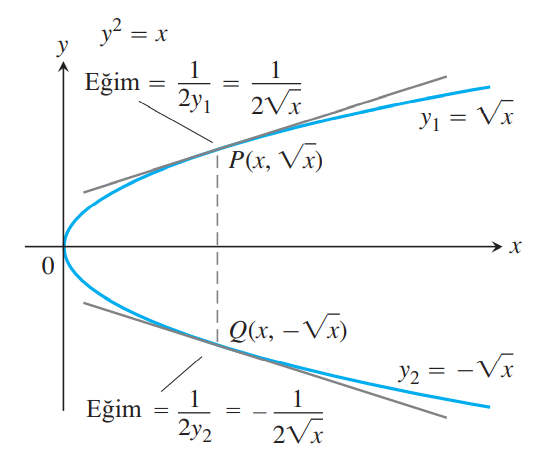
\includegraphics[width=0.5\linewidth]{kapaliturev2.png}
	\caption{$y^2-x=0$, veya genelde yazıldığı şekliyle $y^2-x$ denklemi $x \geq 0$ aralığında $x$'in türevlenebilir iki fonksiyonunu tanımlar. Örnek 1'de, $y^2=x$ denklemini $y$'ye göre çözmeden bu fonksiyonların türevlerinin nasıl alınacağını göstermektedir.}
	\label{fig:ornekresim}
\end{figure}
\begin{figure}[H]
	\centering
	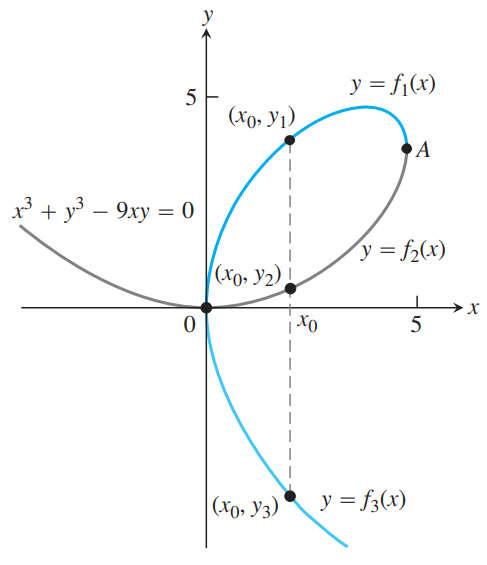
\includegraphics[width=0.5\linewidth]{kapaliturev3.png}
	\caption{$ x^3+y^3-9xy=0$ eğrisi $x$'in tek bir fonksiyonunun grafiği değildir. Ancak, eğri $x$'in fonksiyonlarının grafikleri olan ayrı yaylara bölünebilir. \textit{Folyum} olarak adlandırılan bu özel eğrinin geçimi 1638'den Descartes'e kadar uzanır.}
	\label{fig:ornekresim}
\end{figure}
\begin{ornek}\textit{Bir Çemberin Bir Noktadaki Eğimi}\\
	$x^2+y^2=25$ çemberinin (3,-4) noktasındaki eğimini bulun.
\end{ornek}
\begin{cozum} Çember $x$'in tek bir fonksiyonunun grafiği değildir. İki türevlenebilir fonksiyonun, $y_1=\sqrt{25-x^2}$ ve $y_2=-\sqrt{25-x^2}$ fonksiyonlarının grafiklerinin birleşimidir(Şekil 7.1). (3,-4) noktası $y_2$'nin grafiğinde bulunmaktadır, dolayısıyla eğimi açıkça hesaplayarak bulabiliriz:
	\begin{equation*}
	\frac{dy_2}{dx}|_{x=3}=-\frac{-2x}{2\sqrt{25-x^2}}=-\frac{-6}{2\sqrt{25-9}}=\frac{3}{4}
	\end{equation*}
Ancak, verilen çember denkleminin $x$'e göre kapalı olarak türevini alırsak, problemi daha kolay çözebiliriz:
	\begin{equation*}
	\begin{split}
	\frac{d}{dx}(x^2)+\frac{d}{dx}(y^2)&=\frac{d}{dx}(25)\\
	2x+2y \frac{dy}{dx}&=0\\
	\frac{dy}{dx}&=-\frac{x}{y}
	\end{split}
	\end{equation*}
(3,-4) noktasındaki eğim $\displaystyle - \frac{x}{y}|_{(3,-4)}=-\frac{3}{-4}=\frac{3}{4}$'tür.\\
	Sadece $x$ ekseninin altındaki noktalarda geçerli olan $dy_2/dx$ formülünün aksine, $dy/dx=-x/y$ formülünün çemberin eğiminin bulunduğu her yerde geçerli olduğuna dikkat edin. Ayrıca, türevin sadece bağımsız değişken $x$'i değil, $x$ ve $y$ değişkenlerinin ikisini de içerdiğine dikkat edin.
\end{cozum}\\
Kapalı olarak tanımlanmış başka fonksiyonların türevlerini hesaplamak için, Örnek 7.1.1 ve 7.1.2'deki gibi ilerleriz: $y$'ye $x$'in türevlenebilir kapalı bir fonksiyonu gibi davranır ve bilinen kuralları uygulayarak tanımlayıcı denklemin iki tarafının da türevini alırız.
\begin{ornek}\textit{Kapalı Olarak Türev Alma}\\
	$y^2 = x^2 +\sin{xy}$ ise $ dy/dx$'i bulun.(Şekil 7.4)
\begin{figure}[H]
	\centering
	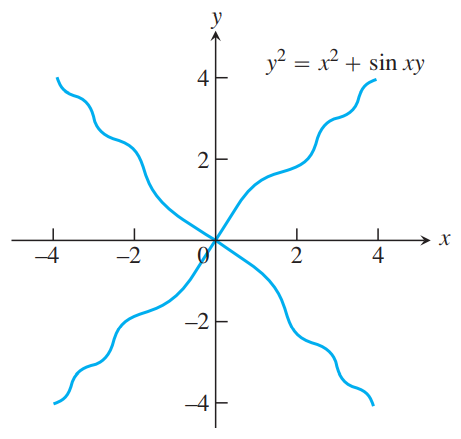
\includegraphics[width=0.5\linewidth]{kapaliturev4.png}
	\caption{Örnek 7.1.3'teki $y^2=x^2+\sin{xy}$'nin denklemi. Örnek, kapalı olarak tanımlanmış bu eğri üzerinde eğimlerin nasıl bulunacağını göstermektedir.}
	\label{fig:ornekresim}
\end{figure}
\end{ornek}
\begin{cozum}
	\begin{equation*}
	\begin{split}
	y^2&=x^2+\sin{xy}\\
	\frac{d}{dx}(y^2)&=\frac{d}{dx}(x^2)+\frac{d}{dx}(\sin{xy})\\
	2y \frac{dy}{dx}&=2x+(\cos{xy})\frac{d}{dx}(xy)\\
	2y \frac{dy}{dx}&=2x+(\cos{xy})\left(y+x \frac{dy}{dx}\right)\\
	2y \frac{dy}{dx}-(\cos{xy})\left(x \frac{dy}{dx}\right)&=2x+(\cos{xy})y\\
	(2y-x \cos{xy}) \frac{dy}{dx}&= 2x+y \cos{xy}\\
	\frac{dy}{dx}&=\frac{2x+y\cos{xy}}{2y-x\cos{xy}}
	\end{split}
	\end{equation*}
$dy/dx$ formülünün, kapalı olarak tanımlanmış eğrinin eğiminin tanımlı olduğu her yere geçerli olduğuna dikkat edin. Ayrıca, türevin sadece bağımsız değişken $x$'i değil, $x$ ve $y$ değişkenlerinin \textit{ikisini} de içerdiğine dikkat edin.
\end{cozum}\\

Kapalı Türev Alma
1. $y$'ye $x$'in türevlenebilir bir fonksiyonu gibi davranarak, denklemin iki tarafının da $x$'e göre türevini alın.
2. $dy/dx$'li terimleri eşitliğin bir tarafında toplayın.
3. $dy/dx$'i çözün.\\

\section{\protect Mercekler, Teğetler ve Normal Doğrular}
Bir merceğe girerken ışığın nasıl yön değiştirdiğini tanımlayan yasada, önemli açılar ışığın merceğe giriş noktasında merceğin yüzeyine dik olan doğruyla yaptığı açılardır(Şekil 7.5'dek $A$ ve $B$ açıları). Bu doğruya giriş noktasında yüzeyin \textit{normali} adı verilir. Şekil 7.5'deki gibi bir merceğin yandan görünüşünde, normal, eğrinin ışığın giriş noktasındaki teğetine dik olan doğrudur.
\begin{figure}[H]
	\centering
	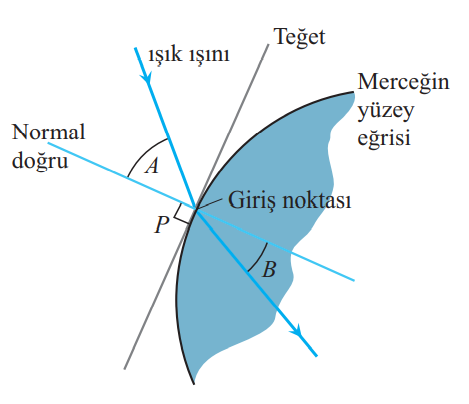
\includegraphics[width=0.5\linewidth]{kapaliturev5.png}
	\caption{Bir ışık ışınının, merceğin yüzeyinden geçerken kırılmasını gösteren mercek profili.}
	\label{fig:ornekresim}
\end{figure}
\begin{ornek}\textit{Descartes Folyumunun Teğeti ve Normali}\\
(2,4) noktasının $x^3+y^3-9xy=0$ eğrisi üzerinde olduğunu gösterin. Sonra, bu eğrinin buradaki teğetini ve normalini bulun(Şekil 7.6).
\begin{figure}[H]
	\centering
	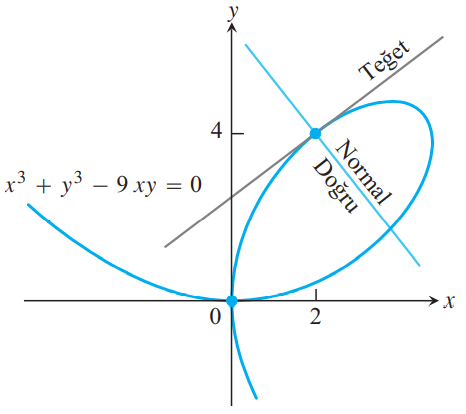
\includegraphics[width=0.5\linewidth]{kapaliturev6.png}
	\caption{Örnek 7.2.1, Descartes folyumunun (2,4)'teki teğetinin ve normalinin denklemlerinin nasıl bulunacağını göstermektedir.}
	\label{fig:ornekresim}
\end{figure}
\end{ornek}
\begin{cozum} (2,4) noktası eğrinin üzerindedir çünkü koordinatları eğrinin denklemini sağlar:\\
$2^3+4^3-9(2)(4)=8+64-72=0$.\\
Eğrinin (2,4)'teki eğimini bulmak için, önce kapalı türev kullanarak $dy/dx$'in formülünü buluruz:
	\begin{equation*}
	\begin{split}
	x^3+y^3-9xy&=0\\
	\frac{d}{dx}(x^3)+\frac{d}{dx}(y^3)-\frac{d}{dx}(9xy)&=\frac{d}{dx}(0)\\
	3x^2+3y^2\frac{dy}{dx}-9\left(x \frac{dy}{dx}+y \frac{dx}{dx}\right)&=0\\
	(3y^2-9x)\frac{dy}{dx}+3x^2-9y&=0\\
	3(y^2-3x)\frac{dy}{dx}&=9y-3x^2\\
	\frac{dy}{dx}&=\frac{3y-x^2}{y^2-3x}
	\end{split}
	\end{equation*}
Sonra $(x,y)=(2,4)$ noktasında türevi hesaplarız:
	\begin{equation*}
	\frac{dy}{dx}|_{(2,4)}=\frac{3y-x^2}{y^2-3x}|_{(2,4)}=\frac{3(4)-2^2}{4^2-3(2)}=\frac{8}{10}=\frac{4}{5}
	\end{equation*}
(2,4) noktasındaki teğet, (2,4)noktasından 4/5 eğimiyle geçen doğrudur:
	\begin{equation*}
	\begin{split}
	y&=4+\frac{4}{5}(x-2)\\
	y&=\frac{4}{5}x+\frac{12}{5}
	\end{split}
	\end{equation*}
Eğrinin (2,4) noktasındaki normali ise burada teğete dik olan doğru, (2,4) noktasından -5/4 eğimiyle geçen doğrudur:
	\begin{equation*}
	\begin{split}
	y&=4-\frac{5}{4}(x-2)\\
	y&=-\frac{5}{4}x+\frac{13}{2}
	\end{split}
	\end{equation*}
\end{cozum}
Kuadratik formül, $y^2-2xy+3x^2=0$ şeklindeki ikinci derece bir denklemden $y$'yi $x$ cinsinden çözmemizi sağlar. Üçüncü dereceden bir denklemin üç kökünü veren, kuadratik formül gibi bir formül vardır fakat çok daha karmaşıktır. Eğer bu formül $x^3+y^3=9xy$ denkleminden $y$'yi $x$ cinsinden çözmek için kullanılsaydı, denklem tarafından tanımlanan üç fonksiyon
	\begin{equation*}
	y=f(x)=\sqrt[3] {-\frac{x^3}{2}+\sqrt{\frac{x^6}{4}-27x^3}}+\sqrt[3] {-\frac{x^3}{2}-\sqrt{\frac{x^6}{4}-27x^3}}
	\end{equation*}
ve
	\begin{equation*}
y=\frac{1}{2}\left[-f(x) \pm \sqrt{-3}\left(\sqrt[3] {-\frac{x^3}{2}+\sqrt{\frac{x^6}{4}-27x^3}}-\sqrt[3] {-\frac{x^3}{2}-\sqrt{\frac{x^6}{4}-27x^3}}\right)\right]
	\end{equation*}
olurdu. Örnek 7.2.1'de kapalı türev almak, $dy/dx$'i yukarıdaki formüllerden herhangi birinden doğrudan doğruya hesaplamaktan çok daha kolaydır. Daa yüksek dereceden denklemlerin tanımladığı eğriler üzerinde eğim bulmak genellikle kapalı türev alma gerektirir.

\section{\protect Yüksek Mertebe Türevler}
Kapalı türev alma daha yüksek mertebeden türevler almak için de kullanılabilir. Aşağıda örnek verilmiştir.
\begin{ornek}\textit{Bir İkinci Mertebe Türevi Kapalı Olarak Bulma}\\

	$2x^3-3y^2=8$ ise $d^2y/dx^2$'yi bulun.
\end{ornek}

\begin{cozum} Başlangıç olarak denklemin iki tarafının da $x$'e göre türevini alarak, $y'=dy/dx$'i buluruz:
	\begin{equation*}
	\begin{split}
	\frac{d}{dx}(2x^3-3y^2)&=\frac{d}{dx}(8)\\
	6x^2-6yy'&=0\\
	x^2-yy'&=0\\
	y'&=\frac{x^2}{y}, y \ne 0
	\end{split}
	\end{equation*}
Şimdi $y''$'nü bulmak için Bölüm Kuralını uygularız.
	\begin{equation*}
	y''=\frac{d}{dx}\left(\frac{x^2}{y}\right)=\frac{2xy-x^2y'}{y^2}=\frac{2x}{y}-\frac{x^2}{y^2}.y'
	\end{equation*}
Son olarak $y''$'nü $x$ ve $y$ cinsinden yazabilmek için $y' = x^2/y$'yi yerine yazarız.
	\begin{equation*}
	y''=\frac{2x}{y}-\frac{x^2}{y^2}\left(\frac{x^2}{y}\right)=\frac{2x}{y}-\frac{x^4}{y^3}, y\ne0
	\end{equation*}
\end{cozum}

\section{\protect Türevlenebilir Fonksiyonların Rasyonel Kuvvetleri}
	\begin{equation*}
	\frac{d}{dx}x^n=nx^{n-1}
	\end{equation*}
kuvvet kuralının $n$ bir tamsayı olduğundan geçerli olduğunu biliyoruz. Şimdi bunu rasyonel $n$ sayısı için de doğru olduğunu göstereceğiz.

\begin{teorem}\textit{Rasyonel Üsler İçin Kuvvet Kuralı}\\
	$p/q$ bir rasyonel sayıysa, $x^{p/q},x^{(p/q)-1}$'in tanım kümesinin her iç noktasında türevlenebilir.
	\begin{equation*}
	\frac{d}{dx}x^{p/q}= \frac{p}{q}x^{(p/q)-1}
	\end{equation*}
\end{teorem}

\begin{ornek}\textit{Rasyonel Üs Kuralını Kullanmak}\\
(a) $\displaystyle \frac{d}{dx}(x^{1/2})=\frac{1}{2}x^{-1/2}=\frac{1}{2\sqrt{x}}$ $x>0$ için\\
(b) $\displaystyle \frac{d}{dx}(x^{2/3})=\frac{2}{3}x^{-1/3}$,		 $x\ne 0$ için\\
(b) $\displaystyle \frac{d}{dx}(x^{-4/3})=\frac{-4}{3}x^{-7/3}$,	    $x\ne 0$ için
\end{ornek}

\begin{ispat}
	$p$ ve $q$, $q>0$ olmak üzere iki tamsayı olsun ve $y=\sqrt[q]{x^p}=x^{p/q}$ olduğunu varsayın. Bu durumda
	\begin{equation*}
	y^q=x^p
	\end{equation*}
olur. $p$ ve $q$'nun ikisi de tamsayı olduğu için (ki tamsayılar için kuvvet kuralını ispatlamıştık), denklemin iki tarafının da $x$'e göre kapalı türevini alabiliriz:
	\begin{equation*}
	qy^{q-1} \frac{dy}{dx}=px^{p-1}
	\end{equation*}
$y \ne 0$ ise, denklemin iki tarafını da $qy^{q-1}$ ile bölüp, $dy/dx$'i bulabiliriz:
	\begin{equation*}
	\begin{split}
	\frac{dy}{dx}&=\frac{px^{p-1}}{qy^{q-1}}\\
	&=\frac{p}{q}. \frac{x^{p-1}}{(x^{p/q})^{q-1}}\\
	&=\frac{p}{q}.\frac{x^{p-1}}{x^{p-p/q}}\\
	&=\frac{p}{q}.x^{(p-1)-(p-p/q)}\\
	&=\frac{p}{q}.x^{(p/q)-1}
	\end{split}
	\end{equation*}
böylece kural ispatlanır.
\end{ispat}
\chapter{\protect İLİŞKİLİ ORANLAR}
Bu bölümde, bazı değişkenlerin değişim oranlarının sorulduğu problemlere bakacağız. Her durumda oran, değiştiği bilinen başka bir değişkenin (belki birkaç değişkenin) değişim oranından hesaplanması gereken bir türevdir. Bunu bulmak için, ilgili değişkenleri birbirine bağlayan bir denklem yazar ve aradığımız oranı bildiğimiz oranlara bağlayan bir denklem elde etmek için türevini alırız. Değişimini ölçebildiğimiz bazı oranlardan kolayca elde edemediğimiz bir oran bulma problemine \textit{iliskili oranlar problemi} denir.

\section{\protect İlişkili Oranlar Denklemleri}
Küresel bir balon içine hava pompaladığımızı varsayın. Balonun hem hacmi hem de yarıçapı zamanla artar. Belirli bir anda balonun hacmi $V$ ve yarıçapı $r$ ise
	\begin{equation*}
	V=\frac{4}{3}\pi r^3
	\end{equation*}
olur. Zincir Kuralını kullanara, İlişkili oranlar denklemi bulmak için türev alırız:
	\begin{equation*}
	\frac{dV}{dt}=\frac{dV}{dr}\frac{dr}{dt}=4\pi r^2 \frac{dr}{dt}
	\end{equation*}
Dolayısıyla, verilen belirli bir zaman anında balonun yarıçapını ve hacmini$dV/dt$ artış oranını biliyorsak, son denklemlerden $dr/dt$'yi çözebilir ve verilen anda yarıçapının ne kadar hızlı arttığını bulabiliriz. Hacmin artış oranının doğrudan ölçümünün, yarıçapın artış oranının doğrudan ölçümünden daha kolay olduğuna dikkat edin. İlişkili oranlar denklemi $dr/dt$'yi $dV/dt$'den hesaplamamızı sağlar\\
Aşağıdaki örnekte gösterildiği gibi, çoğu zaman, bir ilişkili oranlar problemindeki değişkenleri ilişkilendirmenin anahtarı, değişkenler arasındaki geometrik ilişkileri gösteren bir şekil çizmektir.
\begin{ornek}\textit{Bir Tanktan Dışarı Sıvı Pompalamak}\\
	Dikey bir depolama tankının içindeki sıvı seviyesi, sıvıyı 3000 L/dak hızla pompalarsak ne hızla düşecektir?
\end{ornek}

\begin{cozum}
	Bir kısmı dolu dik bir silindir tank çizer ve yarıçapını $r$, sıvının yüksekliğini ise $h$ ile belirtiriz(Şekil 8.1).Sıvının hacmini ise $V$ ile gösteririz.
\begin{figure}[H]
	\centering
	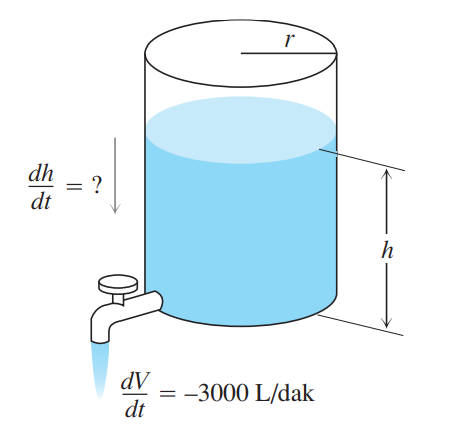
\includegraphics[width=0.5\linewidth]{iliskilioranlar1.png}
	\caption{Bir silindirik tank içindeki sıvı hacminin değişim oranı, tank içindeki sıvı seviyesinin değişim oranına bağlıdır(Örnek 8.1).}
	\label{fig:ornekresim}
\end{figure}
Zaman geçtikçe, yarıçap sabit kalır, fakat $V$ ve $h$ deü,i,r. $V$ ve $h$'yı zamanın türevlenebilir fonksiyonları olarak kabul eder ve zamanı $t$ ile gösteririz. Bize
	\begin{equation*}
	\frac{dV}{dt}=-3000\textit{(Sıvıyı dışarıya 3000L/dak hızla pompalarız. Oran negatiftir, çünkü hacim azalmaktadır.)}
	\end{equation*}
olduğu verilmiştir ve bulmamız istenen
	\begin{equation*}
	\frac{dh}{dt}\textit{(Sıvı seviyesi ne hızla düşecektir?)}
	\end{equation*}
dir. $dh/dt$'yi bulmak için önce $h$'yi $V$'ye bağlayan bir denklem yazarız. Denklem $V$,$r$ ve $h$ için seçilen birimlere bağlıdır. $V$ litre ve $r$ ile $h$ metre ise, silindirin hacmi için uygun denklem
	\begin{equation*}
	V=1000\pi r^2 \frac{dh}{dt}\textit{($r$ sabittir)}
	\end{equation*}
Bilinen $dV/dt=-3000$ değerini yerine koyar ve $dh/dt$'yi çözeriz:
	\begin{equation*}
	\frac{dh}{dt}=\frac{-3000}{1000\pi r^2}=- \frac{3}{\pi r^2}
	\end{equation*}
Sıvı seviyesi $3/(\pi r^2)$ m/dak hızla düşecektir.\\
	$dh/dt = -3/\pi r^2$ denklemi sıvı seviyesinin düşüş oranının tankin yarıçapına nasıl bağlı olduğunu göstermektedir. $r$ küçükse, $dh/dt$ büyük olacaktır; $r$ büyükse, $dh/dt$ küçük olur.
	\begin{equation*}
	\begin{split}
	r=1 m:	\frac{dh}{dt}&=-\frac{3}{\pi}\approx-0.95\textit{m/dak}\\
	r=10 m: \frac{dh}{dt}&=-\frac{3}{100\pi}\approx-0.0095\textit{m/dak}
	\end{split}
	\end{equation*}
\end{cozum}\\





\subsection{\protect İlişkili Oranlar Denklemleri}
1. Bir resim çizin ve değişkenlerle sabitleri isimlendirin. $t$'yi zaman için kullanın. Bütün değişkenlerin zamanın fonksiyonu olduklarını varsayın.\\
2. Sayısal bilgileri yazın (seçtiğiniz sembollari kullanarak).\\
3. Neyi bulmak istediğinizi yazın (genellikle bir türev olarak ifade edilen bir orandır).\\
4. Değişkenleri birbirine bağlayan bir denklem yazın. Bilmek istediğiniz oranı bildiğiniz oranlarla birleştirecek tek bir denklem yazmak için iki veya daha fazla denklemi birleştirmeniz gerekebilir.\\
5. $t$'ye göre \textit{türev} alın. Bilmek istediğiniz oranı değerini bildiğiniz oran ve değişkenler cinsinden ifade edin.\\
6. Hesaplayın. Bilinen değerleri kullanarak bilinmeyen oranı bulun.

\begin{ornek}
	Yerden yukarı doğru yükselen bir sıcak hava balonu kalkış noktasından 500 ft uzaktaki bir tarayıcı ile izlenmektedir. Tarayıcının balonla yaptığı açı $\pi/4$ olduğu anda, açı 0.14 rad/dak. hızıyla artmaktadır. Balon o anda ne hızla yükselmektedir?
\end{ornek}

\begin{cozum}
(1). Bir resim çizin ve sabitlerle değişkenleri isimlendirin(Şekil 8.2) Resimdeki değişkenler\\
	$\theta$=tarayıcının yer ile yaptığı açı(radyan)\\
	$y$= balonun feet olarak yüksekliği\\
dir. $t$ zamanı temsil eder ve $\theta$ ile $y$'nin $t$'nin türevlenebilir fonksiyonları olduğunu varsayarız.
\begin{figure}[H]
	\centering
	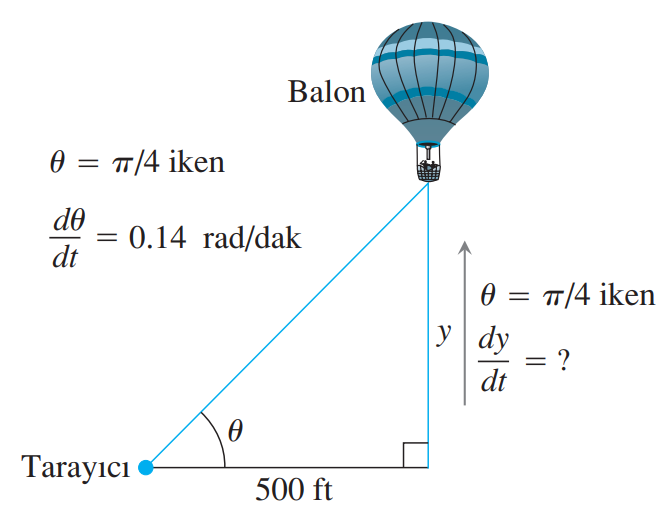
\includegraphics[width=0.5\linewidth]{iliskilioranlar2.png}
	\caption{Balon yüksekliğinin değişim oranı telemetrenin yer ile yaptığı açının değişim oranına bağlıdır(Örnek 8.1.1).}
\end{figure}
Resimdeki tek sabit tarayıcının kalkış noktasına olan uzaklığıdır(500ft). Buna özel bir sembol atamanın gereği yoktur.\\
(2). Diğer sayısal bilgileri yazın.
	\begin{equation*}
	\theta=\frac{\pi}{4} \textit{iken} \frac{d\theta}{dt}=0.14 \textit{rad/dak.}
	\end{equation*}
(3). Neyi bulmamız gerektiğini yazın. $\theta=\pi /4$ iken $dy/dt$'yi istiyoruz.
(4). $y$ ve $\theta$ değişkenlerini ilişkilendiren bir denklem yazın.
	\begin{equation*}
	\frac{y}{500}=\tan{\theta} \textit{(ya da) } y=500 \tan{\theta}
	\end{equation*}
(5). Zincir kuralını kullanarak $t$'ye göre türev alın. Sonuç $dy/dt$'nin $d\theta/dt$ ile ilişkisinin nasıl olduğunu gösterir.
	\begin{equation*}
	\frac{dy}{dt}=500(\sin^2\theta)\frac{d\theta}{dt}
	\end{equation*}
(6). $\theta=\pi /4$ ve $d\theta/dt=0.14$ değerlerini yerine koyun $dy/dt$'yi bulun.
	\begin{equation*}
	\frac{dy}{dt}=500(\sqrt{2})^2(0.14)=140
	\end{equation*}
Söz konusu anda, balon 140 ft/dak hızıyla yükselmektedir.
\end{cozum}

\chapter{\protect LİNEERİZASYON ve DİFERANSİYELLER}
	Bazen fonksiyonlara, özel uygulamalar için istediğimiz hassaslığı veren ve çalışılması daha kolay olan fonksiyonlarla yaklaşımda bulunuruz. Bu bölümde tartışılan yaklaşım fonksiyonlarına \textit{lineerizasyonlar} denir ve teğet doğrularını temel alırlar.\\
Diferansiyeller adı verilen yeni $dx$ ve $dy$ değişkenlerini tanıtacak ve bunları, türevin $dy/dx$ Leibniz gösterimine gerçek bir oran anlamı verecek şekilde tanımlayacağız.  $dy$'yi ölçümlerdeki hatayı ve bir fonksiyonun değişikliklere karşı duyarlılığı ölçmekte kullanacağız. Bu fikirlerin uygulamaları Zincir Kuralını tam ispatını sağlayacaktır(Bölüm 6).
\section{\protect Lineerizasyon}
Şekil 9.1'de göreceğiniz gibi,$y=x^2$ eğrisinin teğeti değme noktası civarında eğriye yakın bulunur. İki tarafta da kısa bir aralıkta, teğet doğrusu üzerindeki $y$ değerleri eğri üzerindeki $y$ değerlerinin oldukça iyi bir yaklaşımını verir. Bu olayı, her iki grafik üzerinde değme noktasına yakından bakarak veya değme noktasının $x$-koordinatı yakınlarında $f(x)$ ile teğeti arasındaki değer farkları tablosuna bakarak görebiliriz. Yerel olarak her türevlenebilir eğri bir doğru gibi davranır.
\begin{figure}[H]
	\centering
	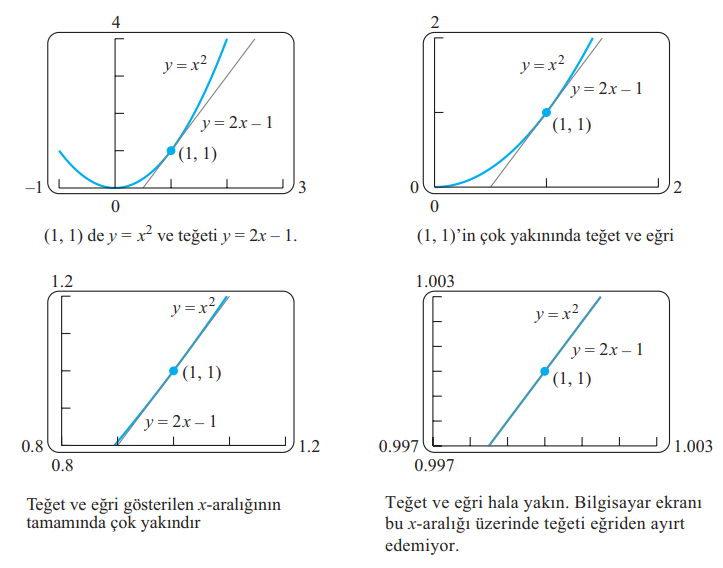
\includegraphics[width=0.87\linewidth]{lineerizasyon1.png}
	\caption{Bir fonksiyonun türevlenebilir olduğu bir noktadaki grafiğini büyüttükçe grafik düzleşir ve teğetine benzerliği artar.}
	\label{fig:ornekresim}
\end{figure}
Genel olarak, $y=f(x)$'in türevlenebilir olduğu bir $x=a$ noktasındaki teğeti(Şekil 9.2) $(a,f(a))$ noktasından geçer, dolayısıyla nokta-eğim denklemi şu şekildedir:
 	\begin{equation*}
	y=f(a)+f'(a)(x-a)
	\end{equation*}
Yani, teğet
	\begin{equation*}
	L(x)=f(a)+f'(a)(x-a)
	\end{equation*}
lineer fonksiyonunun grafiğidir. Doğru $f$'nin grafiğine yakın kaldığı sürece, $L(x)$ $f(x)$'e iyi bir yaklaşım verecektir.
\begin{figure}[H]
	\centering
	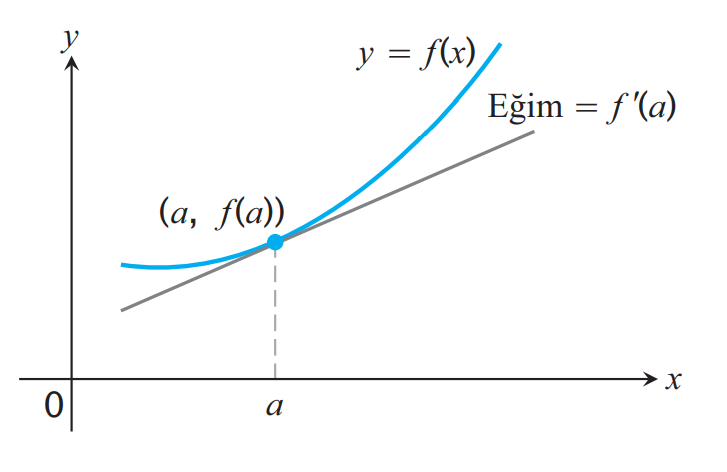
\includegraphics[width=0.5\linewidth]{lineerizasyon2.png}
	\caption{$y=f(x)$ eğrisinin $x=a$ daki teğet doğrusunun denklemi\\ $L(x)=f(a)+f'(a)(x-a)$'dır.}
	\label{fig:ornekresim}
\end{figure}
%BURADAN ÖNCESİ ÇALIŞIYOR DOKUNMA%S
\begin{tanim}
	$f$ fonksiyonu $x=a$'da türevlenebilirse,
	\begin{equation*}
	L(x)=f(a)+f'(a)(x-a)
	\end{equation*}
yaklaştırma fonksiyonu, $f$'nin $a$'daki \textit{lineerizasyonudur}. $f$'ye $L$ tarafından yapılan
	\begin{equation*}
	f(x) \approx L(x)
	\end{equation*}
yaklaşımı $f$'nin $a$'daki \textit{standart lineer yaklaşımıdır}.  $x=a$ noktası yaklaşımın \textit{merkezi}dir.
\end{tanim}
\begin{ornek}\textit{Bir Lineerizasyon Bulmak}\\
$f(x)=\sqrt{1+x}$'in $x=0$'daki lineerizasyonunu bulun(Şekil 9.3)
\begin{figure}[H]
	\centering
	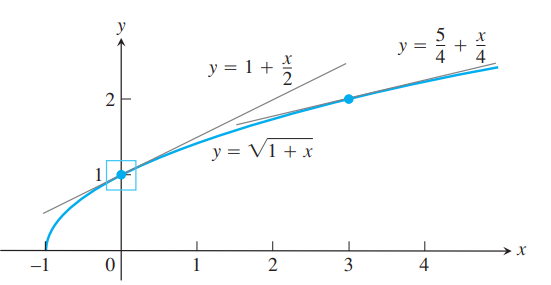
\includegraphics[width=0.5\linewidth]{lineerizasyon3.png}
	\caption{$y=\sqrt{1+x}$'in grafiği ve $x=0$ ve $x=3$'teki lineerizasyonları. Şekil 9.4 de $y$-eksenindeki 1 civarında küçük bir çerçevenin büyütülmüş görüntüsü verilmiştir.}
	\label{fig:ornekresim}
\end{figure}
\end{ornek}
\begin{cozum}
	\begin{equation*}
	f'(x)=\frac{1}{2}(1+x)^{-1/2}
	\end{equation*}
olduğu için, $f(0)=1/2$'dir. Buradan
	\begin{equation*}
	L(x)=f(a)+f'8a)(x-a)=1+\frac{1}{2}(x-0)=1+\frac{x}{2}
	\end{equation*}
bulunur. Şekil 9.4'e bakın.
\begin{figure}[H]
	\centering
	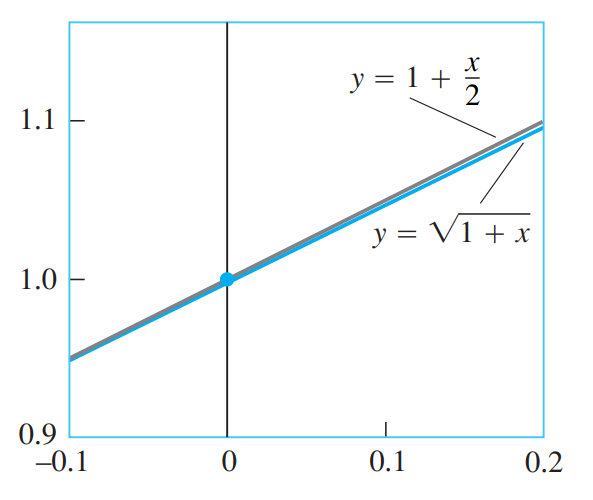
\includegraphics[width=0.5\linewidth]{lineerizasyon4.png}
	\caption{Şekil 9.3'teki çerçevenin büyütülmüş görüntüsü.}
	\label{fig:ornekresim}
\end{figure}
Örnek 9.1.1'deki $\sqrt{1+x}\approx1+(x/2)$ yaklaşımının 0'a yakın $x$'ler için ne kadar doğru olduğuna bakın.\\
Sıfırdan uzaklaştıkça doğruluğu kaybederiz. Örneğin, $x=2$ için, lineerizasyon$\sqrt{3}$ için yaklaşım olarak 2'yi verir ki, bir ondalık basamağa kadar bile doğru değildir.\\
Bu hesaplamalarla lineerizasyonla bütün yapacaklarımızın bir hesap makinesiyle yapılmasının daha iyi olacağı fikrine kapılmayın. Pratikte, asla belirli bir karekökü bulmak için bir lineerizasyon kullanmayız. Bir lineerizasyonun yararı karmaşık bir fonksiyonu bütün bir değer aralığında daha basitiyle değiştirme becerisidir. 0'a yakın $x$ değerlerinde $\sqrt{1+x}$ ile çalışmak zorundaysak ve ortaya çıkacak küçük bir hataya göz yumabilecek durumdaysak $1+(x/2)$ ile çalışabiliriz. Elbette, bu durumda da hatanın ne kadar olduğunu bilmemiz gerekir.
\begin{figure}[H]
	\centering
	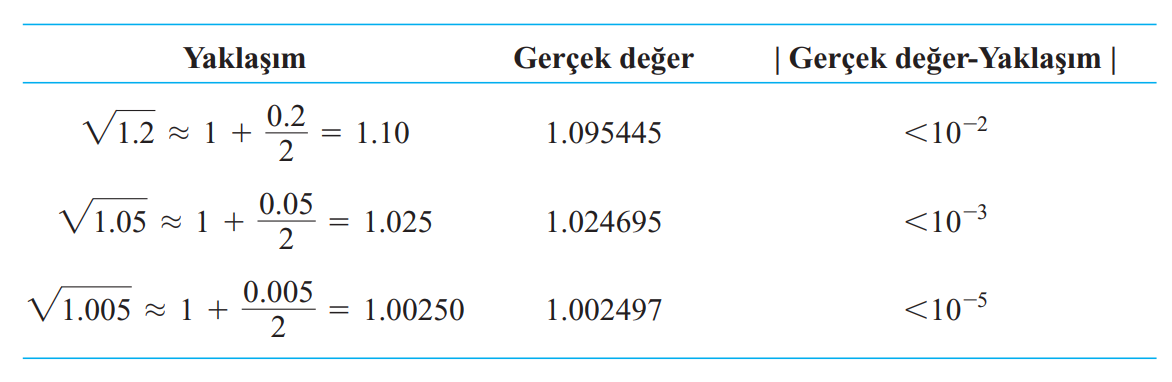
\includegraphics[width=0.9\linewidth]{lineerizasyon5.png}
	\label{fig:ornekresim}
\end{figure}
Normalde bir lineer yaklaşım merkezinde uzakta hassaslığını yitirir. Şekil 9.3'ün gösterdiği gibi, $\sqrt{1+x}\approx1+(x/2)$ yaklaşımı büyük olasılıkla  $x=3$ civarında yararlı olamayacak kadar kaba olacaktır. O noktada, $x=3$'teki lineerizasyona ihtiyacımız vardır.
\end{cozum}
\begin{ornek}\textit{Başka Bir Noktada Bir Lineerizasyon Bulmak}\\
$f(x)=\sqrt{1+x}$'in $x=3$'teki lineerizasyonunu bulun.
\end{ornek}
\begin{cozum}$L(x)$'i tanımlayan denklemi $a=3$'te hesaplarız.
	\begin{equation*}
	f(3)=2, f'(3)=\frac{1}{2}(1+x)^{-1/2}|_{x=3}=\frac{1}{4}
	\end{equation*}
olduğu için,
	\begin{equation*}
	L(x)=2+\frac{1}{4}(x-3)=\frac{5}{4}+\frac{x}{4}
	\end{equation*}
$x=3.2$'de, Örnek 9.1.2'deki lineerizasyon
	\begin{equation*}
	\sqrt{1+x}= \sqrt{1+3.2}\approx \frac{5}{4}+\frac{3.2}{4}=1.250+0.800=2.050
	\end{equation*}
verir, ki bu da gerçek değer $\sqrt{4.2}\approx2.04939$'dan binde birden daha az bir oranda değişir. Örnek 9.1.1'deki lineerizasyon
	\begin{equation*}
	\sqrt{1+x}=\sqrt{1+3.2}\approx1+\frac{3.2}{2}=1+1.6=2.6,
	\end{equation*}
ise gerçek değerden $\% 25$'ten daha fazla fark gösteren bir sonuçtur.
\end{cozum}\\
\section{\protect Diferansiyeller}
Bazen $y$'nin $x$'e göre türevini göstermek için $dy/dx$ Liebniz notasyonunu kullanırız. Görünüşünün tersine, bu bir oran değildir. Şimdi, oranları tanımlı olduğunda türeve eşit olacak olan iki yeni değişken, $dx$ ve $dy$ tanıtacağız.
\begin{tanim}\textit{Diferansiyeller}
	$y=f(x)$ türevlenebilir bir fonksiyon olsun. $dx$ diferansiyeli bağımsız bir değişkendir. $dy$ diferansiyeli
	\begin{equation*}
	dy=f'(x)dx
	\end{equation*}
olarak tanımlanır.
\end{tanim}
Bağımsız değişken $dx$'in aksine, $dy$ değişkeni her zaman bağımlı bir değişkendir. Hem $x$'e hem de $dx$'e bağlıdır. $dx$ belirli bir değerse ve $x$, $f$ fonksiyonunu tanım kümesinde özel bir sayı ise $dy$'nin sayısal değeri tanımlıdır.

\begin{ornek}$dy$\textit{Diferansiyelini Bulmak}\\
(a).$y=x^5+37x$ ise $dy$'yi bulun.\\
(b).$x=1$ ve$dx=0ç2$ ise, $dy$'nin değerini bulun.
\end{ornek}
\begin{cozum}
(a).$dy=(5x^4+37)dx$\\
(b).$dy$'nin ifadesinde $x=1$ ve $dx=0.2$ yazarsak;
	\begin{equation*}
	dy=(5.1^4+37)0.2=8.4
	\end{equation*}
buluruz.\\
\end{cozum}
\begin{figure}[H]
	\centering
	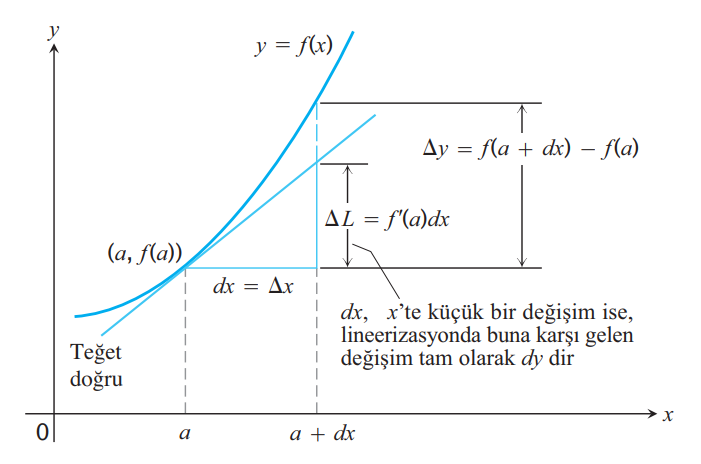
\includegraphics[width=0.7\linewidth]{diferansiyeller1.png}
	\caption{Geometrik olarak, $dy$ diferansiyeli $f$'nin $x=a$'daki lineerizasyonunun $dx=\varDelta x$ değişimine karşı gelen $\varDelta L$ değişimidir.}
	\label{fig:ornekresim}
\end{figure}

Diferansiyellerin geometrik anlamı Şekil 9.5'te gösterlmiştir. $x=a$ ve $dx=\varDelta x$ koyun. Buna karşılık $y=f(x)$'teki değişme
	\begin{equation*}
	\varDelta y= f(a+dx)-f(a)
	\end{equation*}
Buna karşılık $L$ teğet doğrusundaki değişim
	\begin{equation*}
	\begin{split}
	\varDelta L&=L(a+dx)-L(a)\\
	&=\{f(a)+f'(a)[(a+dx)-a]\}-\{f(a)\}\\
	&=f'(a)dx
	\end{split}
	\end{equation*}
dir. Yani, $x=a$ ve $dx=\varDelta x$ olduğunda $f$'nin lineerizasyonundaki değişim tam olarak $dy$ diferansiyelinin değeridir. Bu nedenle $dy$, $x$'te $dx=\varDelta x$ kadar bir değişim meydana geldiğinde, teğet doğrunun buna karşı gelen yükselmesini veya alçalmasını gösterir\\
$dx \ne 0$ ise, $dy$ diferansiyelinin $dx$ diferansiyeline oranı $f'(x)$ türevine eşittir çünkü:
	\begin{equation*}
	dy \div dx = \frac{f'(x)dx}{dx}=f'(x)=\frac{dy}{dx}
	\end{equation*}
olur. Bazen $dy=f'(x)dx$ yerine $df$'e $f$\textit{'nin diferansiyeli} diyerek
	\begin{equation*}
	df=f'(x)dx
	\end{equation*}
yazarız. Örneğin, $f(x)=3x^2-6$ ise
	\begin{equation*}
	df=d(3x^2-6)=6x dx
	\end{equation*}
gibi
	\begin{equation*}
	\frac{d(u+v)}{dx}=\frac{du}{dx}+\frac{dv}{dx}\textit{,   veya   ,}\frac{d(\sin u)}{dx}=\cos u \frac{du}{dx}
	\end{equation*}
gibi her türev formülüne karşılık
	\begin{equation*}
	d(u+v)=du+dv\textit{,   veya   ,}d(\sin u) =\cos{u}u
	\end{equation*}
şeklinde bir diferansiyel form karşılık gelir.
\begin{ornek}\textit{Fonksiyonların Diferansiyellerini Bulmak}\\
(a)  $d(\tan{2x})=\sec^2{2x}d(2x)=2\sec^2{2x}dx$\\
(b)  $\displaystyle d\left(\frac{x}{x+1}\right)=\frac{(x+1)dx-x d(x+1)}{(x+1)^2}=\frac{xdx+dx-xdx}{(x+1)^2}=\frac{dx}{(x+1)^2}$
\end{ornek}
\subsection{\protect Diferansiyellerle Tahmin Etme}
Türevlenebilir $f(x)$ fonksiyonunun bir $a$ noktasındaki değerini bildiğimizi ve bu değerin çok yakınındaki bir $a+dx$ noktasına gittiğimizde nasıl değiştiğini tahmin etmek istediğimizi varsayalım. $dx$ küçükse, Şekil 9.5ten $\varDelta y$'nin yaklaşık olarak $dy$ diferansiyeline eşit olduğunu görebiliriz, çünkü
	\begin{equation*}
	f(a+dx)=f(a)+ \varDelta y,
	\end{equation*}
olduğundan diferansiyel yaklaşımı $dx=\varDelta x$ olmak üzere
	\begin{equation*}
	f(a+dx)\approx f(a)+dy
	\end{equation*}
verir. Böylece, $\varDelta y \approx dy$ yaklaşımı, $f(a)$ biliniyorsa ve $dx$ küçükse $f(a+dx)$'i hesaplamak için kullanılır.
\begin{ornek}\textit{Diferansiyellerle Tahmin Etme}\\
Bir çemberin yarıçapı $r$, $a=10 m$'den 10.1 m'ye artıyor. Çemberin alanı $A$'daki artışı tahmin etmek için $dA$'yı kullanın. Genişletilmiş çemberin alanını tahmin edin ve bunu gerçek alanla karşılaştırın.
\end{ornek}
\begin{cozum}
$A=\pi r^2$ olduğu için, tahmin edilen artış
	\begin{equation*}
	dA=A'(a)dr=2\pi a dr = 2\pi (10)(0.1)=2\pi m^2
	\end{equation*}
bulunur. Böylece,
	\begin{equation*}
	\begin{split}
	A(10+0.1)&\approx A(10)+2\pi \\
	&=\pi(10)^2+2\pi=102\pi
	\end{split}
	\end{equation*}
dir. Yarı çapı 10.1 m olan çemberin alanı yaklaşık olarak 102$\pi m^2$dir.\\
Gerçek alan
	\begin{equation*}
	\begin{split}
	A(10.1)&=\pi(10.1)^2\\
	&=102.01 \pi m^2
	\end{split}
	\end{equation*}
dir. Tahminimizdeki hata $\varDelta A-dA$ farkı olan $0.01 \pi m^2$dir.
\end{cozum}
\subsection{\protect Diferansiyel Yaklaşımındaki Hata}
$f(x)$ fonksiyonu $x=a$ da türevlenebilir olsun ve $x$'teki bir artma $dx=\varDelta x$ olsun. $x$ $a$'dan $a+\varDelta x$'e değişirken $f$'deki değişimi tanımlamanın iki yolu vardır:\\
Gerçek değişim:		$\varDelta f=f(a+ \varDelta x)-f(a)$\\
Diferansiyel tahmin:	$df=f'(a) \varDelta x$\\

$df$'nin $\varDelta f$'e yaklaşımı ne kadar iyidir?\\

Yaklaşımdaki hatayı $\varDelta f$'ten $df$'i çıkararak buluruz:
	\begin{equation*}
	\begin{split}
	\textit{Yaklaşım hatası}&= \varDelta f- df\\
	&=\varDelta f-f'(a)\varDelta x\\
	&=f(a+\varDelta x)-f(a)-f'(a)\varDelta x\\
	&=\left( \frac{f(a+\varDelta x)-f(a)}{\varDelta x}-f'(a)\right).\varDelta x
	\end{split}
	\end{equation*}
$\displaystyle \left( \frac{f(a+\varDelta x)-f(a)}{\varDelta x}-f'(a)\right)=\epsilon$ dersek eşitliğimiz $\epsilon.\varDelta x$ olur.\\
$\varDelta x \rightarrow 0$ iken
	\begin{equation*}
	\frac{f(a+ \varDelta x)-f(a)}{\varDelta x}
	\end{equation*}
fark oranı $f'(a)$'ya yaklaşır ($f'(a)$'nın tanımını hatırlayın), dolayısıyla parantez içindeki değer çok küçük bir sayı haline gelir (bu yüzden ona $\epsilon$ dedik). Aslında, $\varDelta x \rightarrow 0$ iken $\epsilon \rightarrow 0$'dır. $\varDelta x$ küçük ise $\epsilon \varDelta x$ yaklaşım hatası daha küçüktür.\\
$\varDelta f$'e gerçek değişim, $f'(a) \varDelta x$'e tahmini değişim ve $\epsilon \varDelta x$'e de hata dersek,
	\begin{equation*}
	\varDelta f = f'(a) \varDelta x + \epsilon \varDelta x
	\end{equation*}
olur. Hatanın tam olarak ne kadar küçük olduğunu bilmememize ve bunun üzerine daha fazla ilerleme yapmayacak olmamıza rağmen, burada bahsedilmeye değer bir şey vardır, yani denklemin aldığı form şu şekildedir:\\

$x=a$ \textit{yakınında} $y=f(x)$\textit{'teki değişim}\
	$y=f(x)$ $x=a$'da türevlenebiliyor ve $x$ $a$'dan $a+\varDelta x$'e değişiyorsa, $f$'deki $\varDelta y$ değişimi
	\begin{equation}
	\varDelta y=f'(a) \varDelta x + \epsilon \varDelta x
	\end{equation}
formunda bir denklemle verilir. Burada $\varDelta x \rightarrow 0$ iken $\epsilon \rightarrow 0$ olur.\\

(9.1) denklemi Zincir Kuralının ispatını başarılı bir şekilde sonlandırmamızı sağlar.

\begin{ispat}\textit{Zincir Kuralının İspatı}\\
Amacımız $f(u)$ $u$'nun türevlenebilir bir fonksiyonu ve $u=g(x)$ de $x$'in türevlenebilir bir fonksiyonu ise, $y=f(g(x))$ bileşkesi $x$'in türevlenebilir bir fonksiyonudur.\\
	Daha açık olarak, $g$ $x_0$'da türevlenebiliyorsa ve $f$ de $g(x_0)$'da türevlenebiliyorsa, bileşke $x_0$'da türevlenebilir:
	\begin{equation*}
	\frac{dy}{dx}|_{x=x_0}=f'(g(x_0)).g'(x_0)
	\end{equation*}
$\varDelta x$ $x$'in bir artımı ve $\varDelta u$ ve $\varDelta y$ de $u$ ve $y$'de buna karşılık gelen artırımlar olsun. Denklem (9.1)i uygulamakla
	\begin{equation*}
	\varDelta u=g'(x_0) \varDelta x + \epsilon_1 \varDelta x=(g'(x_0)+\epsilon_1)\varDelta x
	\end{equation*}
elde ederiz. Burada $\varDelta x \rightarrow 0$ iken $\epsilon_1 \rightarrow 0$ olur. Aynı şekilde,
	\begin{equation*}
	\varDelta y=f'(u_0) \varDelta u + \epsilon_2 \varDelta u =(f'(u_0)+\epsilon_2)\varDelta u
	\end{equation*}
olur ve yine $\varDelta u \rightarrow 0$ iken $\epsilon_2 \rightarrow 0$'dır. Ayrıca $\varDelta x \rightarrow 0$ iken $\varDelta u \rightarrow 0$ olduğuna dikkat edin. $\varDelta u$ ve $\varDelta y$ denklemlerini birleştirmek\\
	\begin{equation*}
	\varDelta y=(f'(u_0)+\epsilon_2)(g'(x_0)+\epsilon_1)\varDelta x
	\end{equation*}
verir, dolayısıyla
	\begin{equation*}
	\frac{\varDelta y}{\varDelta x}=f'(u_0)g'(x_0)+\epsilon_2 g'(x_0)+f'(u_0)\epsilon_1+\epsilon_2\epsilon_1
	\end{equation*}
olur. $\varDelta x$ sıfıra giderken $\epsilon_1$ ve $\epsilon_2$ de sıfıra gittiği için, denklemin sağ tarafındaki dört terimin üçü limitte sıfır olur ve
	\begin{equation*}
	\frac{dy}{dx}|_{x=x_0}=\lim_{\varDelta x \rightarrow 0} \frac{\varDelta y}{\varDelta x}=f'(u_0)g'(x_0)=f'(g(x_0)).g'(x_0)
	\end{equation*}
kalır. Böylece ispat tamamlanmış olur.
\end{ispat}
\section{\protect Değişime Karşı Duyarlılık}
$df=f'(x)dx$ denklemi $f$'nin çıktısının farklı $x$ değerleri için girdilerdeki değişikliklere ne kadar duyarlı olduğunu göstermektedir. $f'$'nün $x$'teki değeri ne kadar büyükse, $dx$'e verilen bir değişikliğin etkisi de o kadar büyüktür. Bir $a$ noktasından yakınındaki bir $a+dx$ noktasına giderken $f$'deki değişimi üç şekilde tanımlayabiliriz.
\begin{figure}[H]
	\centering
	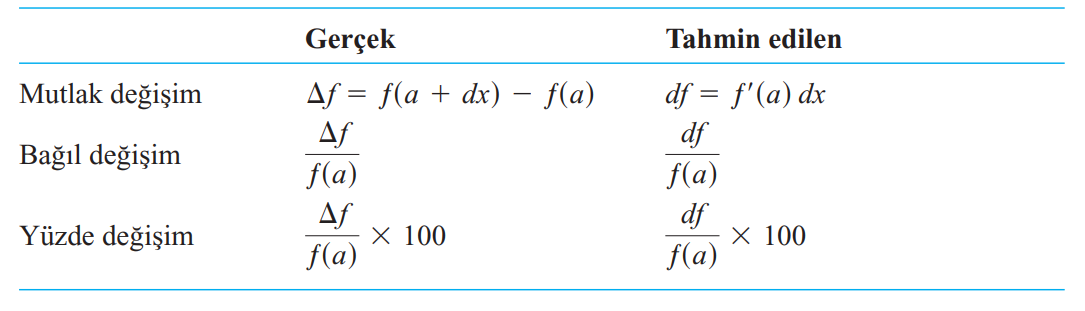
\includegraphics[width=0.9\linewidth]{degisimduyar.png}
	\label{fig:ornekresim}
\end{figure}
\begin{ornek} \textit{Bir Kuyunun Derinliğini hesaplamak}\\
$s=16t^2$ denkleminden, attığınız ağır bir taşın suya ne kadar zamanda düştüğünü ölçerek bir kuyunun derinliğini hesaplamak istiyorsunuz. Hesabınız zamanı ölçerken yapacağını 0.1 sn'lik bir hataya ne kadar duyarlıdır?
\end{ornek}
\begin{cozum}
	\begin{equation*}
	ds=32t dt
	\end{equation*}
denkleminde $ds$'nin boyutu $t$'nin ne kadar büyük olduğuna bağlıdır.\\
Eğer $t=2$ sn ise, $dt=0.1$'in yol açacağı hata sadece
	\begin{equation*}
	ds=32(2)(0.1)=6.4 ft.
	\end{equation*}
olacaktır. Üç saniye sonra, $t=5$ sn iken, aynı $dt$'nin yol açtığı hata
	\begin{equation*}
	ds=32(5)(0.1)=16ft
	\end{equation*}
olacaktır. Kuyunun tahmin edilen derinliğinin gerçek derinliğinden farkı, zaman ölçümündeki verilen bir hata için, atılan aşağıdaki suya çarpmasına kadar geçen süre arttıkça büyür.
\end{cozum}



%sonuç bölümü
\chapter{\protect TARTIŞMA, SONUÇ VE ÖNERİLER}

Türev, doğadaki bir çok olayı tanımlamamıza ve birbirleriyle ilişkilendirilmesine yardımcı olan bir araçtır. Hangi değişkenleri seçtiğimize bağlı olarak, günlük hayattaki karşılaştığımız her şeyde hatta karşılaşmadıklarımızda bile anlam kazandırır, yorum yaptırır. Yapılan bu yorumlar için de günümüze kadar birikerek gelmiş ispatlar yardımıyla doğruluğuna ve mantıklılığına karar veririz. Sonuç olarak bazı şeyler bağımlı, bazı şeyler de bağımsız olarak değişmekte ve türev bu değişimlerin birbirlerine göre durumlarını bilime dayalı ve akla uygun olarak gösteren bir araçtır.
\begin{thebibliography}{99}
\bibitem{Calculus} Thomas Calculus Onbirinci Baskı, 11. Baskıdan çeviri 1. Baskı - Ağustos 2009 - İSTANBUL,147-242s.)
\end{thebibliography}



%burada örnek kaynaklar listelenmiştir. kendi kaynaklarınızı buradakilerle değiştiriniz.
\end{document}